\documentclass[svgnames,t]{beamer}
\usepackage[english]{babel}
\usepackage{%
    fontspec,
    mathabx,
    pifont,
    etoolbox,
    listings,
    lstautogobble,
    tikz,
    multicol,
    moresize,
    relsize,
    array,
    booktabs,
    makecell
}

\setsansfont{Yanone Kaffeesatz}[
    UprightFont     = *-Regular ,
    BoldFont        = *-Bold ,
    BoldItalicFont  = *-Bold ,
    BoldSlantedFont = *-Bold ,
    ItalicFont      = *-Light ,
    SlantedFont     = *-Light ,
    SmallCapsFont   = *-Thin
]

%\setmonofont{Latin Modern Mono Prop}

\usetikzlibrary{
    overlay-beamer-styles,
    calc,
    positioning,
    decorations.pathreplacing,
    backgrounds, shadings,
    shapes
}

\tikzset{
    %Displaying keys
    onslide/.code args={<#1>#2}{\only<#1>{\pgfkeysalso{#2}}}, % \pgfkeysalso doesn't change the path
    scope on/.style={
        every node/.append style={visible on=#1},
        every path/.append style={visible on=#1}
    },
    %Path ending shapes
    to/.style={->,>=stealth},
    from/.style={<-,>=stealth},
    fromto/.style={<->,>=stealth},
    shorter/.style 2 args={shorten <= #1, shorten >= #2},
    %Hexagons
    hexagon/.style n args={3}{double arrow, double arrow head extend=0cm, inner sep=3pt, draw=#1, fill=#2, text=#3, thick},
    hexagon/.default={black}{gray!20}{black},
    hexagonOne/.style={hexagon={#1}{#1!30}{#1}},
    hexagonTwo/.style 2 args={hexagon={#1}{#1!#2}{#1}},
    hexagonThree/.style n args={3}{hexagon={#1}{#1!#2}{#3}},
    hexagonShade/.style n args={3}{double arrow, double arrow head extend=0cm, inner sep=3pt, thick, draw=#1, left color=#2, right color=#3},
    %General text element
    Shape/.style n args={3}{draw=#1, fill=#2, text=#3},
    genShape/.style 2 args={#1, inner sep=3pt, draw=#2, fill=#2!20, text=#2, thick},
    halo/.style={preaction={draw, #1, line width=7, -}},
}
%Colors for listings
\colorlet{background-color}{gray!20}
\colorlet{basic-color}{black}
\colorlet{keywords-color}{Goldenrod}
\colorlet{comment-color}{red!95!black}
\colorlet{strings-color}{ForestGreen}
\colorlet{builtins-color}{MediumBlue!90!black}
\colorlet{functions-color}{NavyBlue}
\colorlet{variables-color}{DarkOrange}
\colorlet{environment-color}{Gray}
\colorlet{external-color}{SteelBlue}

% https://tex.stackexchange.com/a/34000
\makeatletter
\lst@Key{countblanklines}{true}[t]%
    {\lstKV@SetIf{#1}\lst@ifcountblanklines}

\lst@AddToHook{OnEmptyLine}{%
    \lst@ifnumberblanklines\else%
       \lst@ifcountblanklines\else%
         \advance\c@lstnumber-\@ne\relax%
       \fi%
    \fi}
\makeatother

%listings set
\lstdefinestyle{MyBash}{
backgroundcolor=\color{background-color}, % choose the background color; you must add \usepackage{color} or \usepackage{xcolor}
breakatwhitespace=false,            % sets if automatic breaks should only happen at whitespace
breaklines=true,                    % sets automatic line breaking
captionpos=b,                       % sets the caption-position to bottom
deletekeywords={...},               % if you want to delete keywords from the given language
escapeinside={@|}{|@},              % if you want to add LaTeX within your code
extendedchars=true,                 % lets you use non-ASCII characters; for 8-bits encodings only,
                                    % does not work with UTF-8
frame=single,                       % adds a frame around the code
framerule=0pt,                      % Width of the frame rule
framesep=3pt,                       % separation around text
linewidth=\textwidth,               % defines the base line width for listings
xleftmargin=6mm,                    % Margin left
xrightmargin=6mm,                   % Margin right
numbers=left,                       % where to put the line-numbers; possible values are (none, left, right)
numberblanklines=false,             % suppress numbers on empty lines
countblanklines=false,              % NOT standard! Avoid counting empty lines: https://tex.stackexchange.com/a/34000
numbersep=8pt,                      % how far the line-numbers are from the code
numberstyle=\tiny\color{black},     % the style that is used for the line-numbers
rulecolor=\color{black},            % if not set, the frame-color may be changed on line-breaks within not-black text
                                    % (e.g. comments (green here))
showspaces=false,                   % show spaces everywhere adding particular underscores; it overrides 'showstringspaces'
showstringspaces=false,             % underline spaces within strings only
showtabs=false,                     % show tabs within strings adding particular underscores
stepnumber=1,                       % the step between two line-numbers. If it's 1, each line will be numbered
tabsize=2,                          % sets default tabsize to 2 spaces
title=\lstname,                     % show the filename of files included with \lstinputlisting; also try caption instead of title
%
%Base style for this presentation 
keepspaces=true,                    % keeps spaces in text, useful for keeping indentation of code
                                    % (possibly needs columns=flexible)
language=bash,
basicstyle=\ttfamily\scriptsize\color{basic-color},
keywordstyle=\color{keywords-color},
stringstyle=\color{strings-color},
commentstyle=\color{comment-color},
morestring=[b][\color{strings-color}]{"},
morestring=[d][\color{strings-color}]{'},
moredelim=[is][\color{basic-color}]{|+}{+|}, % I will use this for terminal output
literate={`}{\textasciigrave}1, % https://tex.stackexchange.com/a/466224/128737
literate={~}{{\textasciitilde}}1,
% literate=% literate={<replace>}{<replacement text>}{<width>}
%   {\#define}{{{\color{CarnationPink}\#define}}}{6}
%   {\#include}{{{\color{CarnationPink}\#include}}}{7},
alsoletter=0123456789![]/\{\}.:+, % This to mark the symbols in keyword/emph[5] to be highlighted (otherkeywords does not work i.e. it highlights also in comments!) -> manual at page 45
morekeywords={if, then, else, elif, fi, case, esac, for, select, while, until, do, done, in, function, time, [[, ]], \{, \}, !, coproc}, %https://askubuntu.com/a/513712
emph=[1]{CreateListOfFiles, LevelOne, LevelTwo, LevelThree, Test, SecondsToTimeStringWithDays, ExampleFunction,
         ExampleFunction_implementation, ExtractColumnFromFile, CalculateSizeOfFiles, ReportOnLargestDirectories,
         CountTill5From, FifthElementOf, CreateAuxiliaryFiles, CleanAuxiliaryFiles, Failure, FailureMsg, Simulation},
emphstyle=[1]{\color{functions-color}}, %Functions
emph=[2]{variableName, invisibleVariable, prefix, day, today, song, aVar, bVar, langRegex, deadline, now,
         index, file, fgbg, color, reference, files, array, message, entry, index, dict, key, flag, line, inputTime,
         days, hours, minutes, seconds, globalVar, pid, extglobSet, counter, filename, extension},
emphstyle=[2]{\color{variables-color}}, %Variables
emph=[4]{PATH, SHELL, IFS, BASH_ALIASES, BASH_REMATCH, PS3, REPLY, HOME, LANGUAGE, EDITOR, PIPESTATUS, PWD, FUNCNEST,
         DIRSTACK, PWD, OLDPWD, SHELLOPTS, BASHOPTS, TIMEFORMAT, COMP_CWORD, COMP_LINE, COMP_POINT, COMP_TYPE, COMP_KEY,
         COMP_WORDBREAKS, COMP_WORDS, COMPREPLY, INPUTRC},
emphstyle=[4]{\color{environment-color}}, %Environment variables
emph=[5]{alias, bg, bind, break, builtin, cd, command, compgen, complete, continue, declare, dirs, disown, echo, enable, eval,
         exec, exit, export, false, fc, fg, getopts, hash, help, history, jobs, kill, let, local, logout, popd, printf, pushd, pwd,
         read, readonly, return, set, shift, shopt, source, suspend, test, times, trap, true, type, typeset, ulimit, umask,
         % case, if, until, while  % <--- these built-in are keywords and I leave them highlighted as such
         unalias, unset, wait, :, ., [, ]},
emphstyle=[5]{\color{builtins-color}}, %Shell built-in
emph=[6]{man, apropos, ls, rm, g++, chmod, cp, awk, sed, cut, perl, args, date, grep, sleep, tput, seq, cat, wc, sort, tail,
         head, sdiff, tar, mktemp, mkdir, ps, emacs, systemd, timeout, parallel, xargs, gnuplot, pdflatex, vi, ping, bash,
         egrep, shuf, stat, find, fgrep, bc, tr, paste, expr, diff, touch},
emphstyle=[6]{\color{external-color}}, %(External) commands
emph=[7]{},
emphstyle=[7]{\color{variables-color}}, %Class for local variables (usually with bad names)
emph=[8]{},
emphstyle=[8]{\color{builtins-color}}, %Class for local commands (usually with bad names)
%
%Additional customizations
belowskip=-7mm,
aboveskip=3pt,
autogobble=true, % lstautogobble needed!
}

\lstnewenvironment{Bash}[1][] %I will rarely use this because putting a $ in it as prompt breaks down TeXclipse highlight syntax!
    {\lstset{style=MyBash, #1}}
    {}

\def\bash{\lstinline[style=MyBash, basicstyle=\ttfamily\color{black}]}

%This additional style is to just print odd numbers (NOTE: style keyword can be repeated and it is cumulative!)
\lstdefinestyle{oddnumbers}{
    stepnumber=2,
    firstnumber=0,
    numberstyle={\tiny\color{black}\ifodd\value{lstnumber}\relax\else\refstepcounter{lstnumber}\fi\tiny\color{black}\ifodd\value{lstnumber}\relax\else\refstepcounter{lstnumber}\fi}
}

%This additional style is to just print odd numbers (NOTE: style keyword can be repeated and it is cumulative!)
\lstdefinestyle{smaller}{
    basicstyle={\linespread{1.2}\ttfamily\ssmall\color{basic-color}}
}

\newcommand<>{\tc}[2]{\textcolor#3{#1}{#2}}
\newcommand{\tikzmark}[1]{\tikz[overlay,remember picture, baseline=-0.5ex] \node at (0,0) (#1) {};}
\newcommand{\URLsymbol}[2][white]{%
    \begin{tikzpicture}[every path/.style={line width=3, rounded corners, #2}]
        \pgfmathsetmacro{\longSide}{0.9}
        \pgfmathsetmacro{\shortSide}{0.3}
        \draw[rotate=45, xshift=0.5*\longSide cm]       (0,0) rectangle (\longSide, \shortSide);
        \draw[rotate=45, halo=#1, #2!50]                   (0,0) rectangle (\longSide, \shortSide);
        \draw[rotate=45, halo=#1, xshift=0.5*\longSide cm] (0, 0.5*\shortSide) -- (0,0) -- (\longSide, 0) -- (\longSide, 0.5*\shortSide);
    \end{tikzpicture}
}
\NewDocumentCommand{\URL}{ O{black} m m O{BGLIGHT} }%
{%
    \raisebox{-0.4ex}{\resizebox{!}{2ex}{\URLsymbol[#4]{#1}}}{\href{#2}{\textcolor{#1}{#3}}}
}

\NewDocumentCommand{\addSection}{ m O{} m m }%
{%
    \setbeamertemplate{section page}[Iceland][#2]{#3}{#4}
    \section{#1}
}

\makeatletter
\newcommand*\keystroke[1]
{%
    \begin{tikzpicture}[baseline=($(key.base)!0.8!(key.south)$), very thin]%
        \pgfmathsetlengthmacro{\textHeight}{0.9*\f@size}
        \pgfmathsetlengthmacro{\textHeightPlus}{1.25*\textHeight}
        \pgfmathsetlengthmacro{\roundedSmall}{0.2}
        \pgfmathsetlengthmacro{\roundedLarge}{0.4}
        \pgfmathsetlengthmacro{\dl}{0.5\pgflinewidth}
        \node[font=\sffamily, inner xsep=2pt, inner ysep=1pt] (text) {\scalebox{1.2}[0.75]{\textsmaller[2]{#1\strut}}};
        \node[rounded corners=\roundedLarge, minimum size=\textHeight, anchor=north west] (key) at (text.north west){};
        \node[rounded corners=\roundedSmall, minimum size=\textHeightPlus] (frame) at ($(key.center)!0.05!(key.south)$){};
        \path coordinate (keyNW) at ($(key.north west)+(\roundedLarge,-\dl)$)
              coordinate (keyNE) at ($(key.north east)-(\roundedLarge,+\dl)$)
              coordinate (keyEN) at ($(key.north east)-(-\dl,\roundedLarge)$)
              coordinate (keyES) at ($(key.south east)+(+\dl,\roundedLarge)$)
              coordinate (keySE) at ($(key.south east)-(\roundedLarge,+\dl)$)
              coordinate (keySW) at ($(key.south west)+(\roundedLarge,-\dl)$)
              coordinate (keyWS) at ($(key.south west)+(+\dl,\roundedLarge)$)
              coordinate (keyWN) at ($(key.north west)-(-\dl,\roundedLarge)$)
              coordinate (frameNW) at ($(frame.north west)+(\roundedSmall,-\dl)$)
              coordinate (frameNE) at ($(frame.north east)-(\roundedSmall,+\dl)$)
              coordinate (frameEN) at ($(frame.north east)-(+\dl,\roundedSmall)$)
              coordinate (frameES) at ($(frame.south east)+(-\dl,\roundedSmall)$)
              coordinate (frameSE) at ($(frame.south east)-(\roundedSmall,-\dl)$)
              coordinate (frameSW) at ($(frame.south west)+(\roundedSmall,+\dl)$)
              coordinate (frameWS) at ($(frame.south west)+(+\dl,\roundedSmall)$)
              coordinate (frameWN) at ($(frame.north west)-(-\dl,\roundedSmall)$);
        \foreach \n in {NW,NE,EN,ES,SE,SW,WS,WN}{
            \draw[line cap=round, ultra thin] (key\n) -- (frame\n);
        }
        \begin{scope}[on background layer]
            \node[draw, rounded corners=\roundedSmall, minimum size=\textHeightPlus, fill=fg] at ($(key.center)!0.05!(key.south)$){};
            \node[draw, rounded corners=\roundedLarge, lower right=gray!20, lower left=gray!50, upper right=gray!50, upper left=gray!80, minimum size=\textHeight, anchor=north west] at (text.north west){};
            \fill [gray!70!bg] (keyNW) -- (keyNE) -- (frameNE) -- (frameNW) -- cycle;
            \fill [gray!50!bg] (keyWS) -- (keyWN) -- (frameWN) -- (frameWS) -- cycle;
            \fill [gray!30!bg] (keyES) -- (keyEN) -- (frameEN) -- (frameES) -- cycle;
            \fill [gray!10!bg]  (keySW) -- (keySE) -- (frameSE) -- (frameSW) -- cycle;
        \end{scope}
  \end{tikzpicture}%
}
\makeatother

\newcommand{\Remark}[2][1mm]
{%
    \hspace{#1}{\tiny\{~#2~\}}%
}

\newcommand{\FrameRemark}[2][1-]%
{%
    \begin{tikzpicture}[remember picture, overlay]
        \node[font=\tiny, anchor=south, visible on=<#1>] at (current page.south) {#2};
    \end{tikzpicture}
}

\newcommand{\MakeEnumerateBox}[1]%
{%
    \hbox{%
      \usebeamerfont*{item projected}%
      \usebeamercolor[bg]{item projected}%
      \vrule width2.25ex height1.85ex depth.4ex%
      \hskip-2.25ex%
      \hbox to2.25ex{%
        \hfil%
        \color{fg}#1%
        \hfil}%
    }%
}

\renewcommand{\checkmark}[1][PS]{\tc{#1}{\ding{51}}}
\newcommand{\crossmark}[1][PT]{\tc{#1}{\ding{55}}}

\def\quizOverlay{1}
\newcounter{QuizNumber}
\resetcounteronoverlays{QuizNumber}% To avoid the counter being increased by overlays
\newenvironment{quiz}[2][1]{%
    \edef\tmpNumber{\numexpr #1 +1\relax}%
    \gdef\quizOverlay{\the\tmpNumber}%
    \stepcounter{QuizNumber}%
    \medskip%
    % mbox to avoid newline after hbox of enumerate
    \mbox{\MakeEnumerateBox{\theQuizNumber}}\enspace #2%
    \begin{itemize}%
}{%
    \end{itemize}%
    \bigskip%
}

\newcommand{\wrongChoice}[1]%
{%
    \item[\alt<\quizOverlay->{\crossmark}{$\bullet$}] #1
}

\newcommand{\correctChoice}[1]%
{%
    \item[\alt<\quizOverlay->{\checkmark}{$\bullet$}] #1
}

\graphicspath{{Figures/}{Figures/Iceland/}}
\makeatletter
\newif\ifgraphicexist

\catcode`\*=11
\newcommand\IfImageCanBeIncluded[1]{% Taken from https://tex.stackexchange.com/a/567990/128737
    \begingroup
        \global\graphicexisttrue
        \ifx\detokenize\@undefined\else
            \edef\Gin@extensions{\detokenize\expandafter{\Gin@extensions}}%
        \fi
        \let\input@path\Ginput@path
        \expandafter\filename@parse\expandafter{#1}%
        \ifx\filename@ext\Gin@gzext
            \expandafter\filename@parse\expandafter{\filename@base}%
            \ifx\filename@ext\relax
                \let\filename@ext\Gin@gzext
            \else
                \edef\Gin@ext{\Gin@ext\Gin@sepdefault\Gin@gzext}%
            \fi
        \fi
        \ifx\filename@ext\relax
            \@for\Gin@temp:=\Gin@extensions\do{%
                \ifx\Gin@ext\relax
                    \Gin@getbase\Gin@temp
                \fi}%
        \else
            \Gin@getbase{\Gin@sepdefault\filename@ext}%
            \ifx\Gin@ext\relax
                \global\graphicexistfalse
                \let\Gin@savedbase\filename@base
                \let\Gin@savedext\filename@ext
                \edef\filename@base{\filename@base\Gin@sepdefault\filename@ext}%
                \let\filename@ext\relax
                \@for\Gin@temp:=\Gin@extensions\do{%
                    \ifx\Gin@ext\relax
                        \Gin@getbase\Gin@temp
                    \fi}%
                    \ifx\Gin@ext\relax
                        \let\filename@base\Gin@savedbase
                        \let\filename@ext\Gin@savedext
                    \fi
                \fi
                \ifx\Gin@ext\relax
                    \global\graphicexistfalse
                    \def\Gin@base{\filename@area\filename@base}%
                    \edef\Gin@ext{\Gin@sepdefault\filename@ext}%
                \fi
        \fi
        \ifx\Gin@ext\relax
            \global\graphicexistfalse
        \else
        \@ifundefined{Gin@rule@\Gin@ext}%
            {\global\graphicexistfalse}%
            {}%
        \fi
        \ifx\Gin@ext\relax 
            \gdef\imageextension{unknown}%
        \else
            \xdef\imageextension{\Gin@ext}%
        \fi 
    \endgroup 
    \ifgraphicexist
        \expandafter \@firstoftwo
    \else
        \expandafter \@secondoftwo
    \fi
}
\catcode`\*=12
\makeatother

% Compile with or without photos
\newif\ifCompileWithPhotos
\CompileWithPhotostrue

% Compile with or without photos
\newif\ifAddLinkToTOC
\AddLinkToTOCtrue

\mode<presentation>
{
    \usetheme{Relax}
    \defbeamertemplate{footline}{Empty}{}
    \setbeamersize{text margin left=8mm,text margin right=8mm}
    %\setbeamerfont{section title}{size=\Huge}
    \defbeamertemplate*{section page}{Iceland}[3][]
    {
        \begin{tikzpicture}[overlay,remember picture, every node/.style={inner sep=0pt}]
            \usebeamercolor{section page background canvas}
            \fill[bg] (current page.south west) rectangle (current page.north east);
            \node[text depth=0.5ex, anchor=west] () (sectionTitle) at ($(current page.north west)+(5mm,-8mm)$)
                  {\usebeamerfont{section title}\usebeamercolor[fg]{section title}\insertsectionhead};
            \node[anchor=north east, inner sep=0] (plan) at ($(current page.north east)-(1mm,1mm)$) {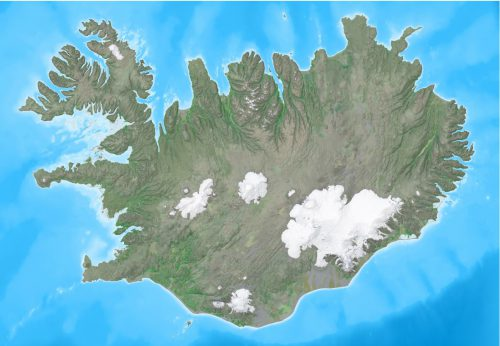
\includegraphics[width=0.21\textwidth, clip, trim=0 0 0 1mm]{Map}};
            \node[anchor=north] (photo) at ($(plan.south west)!0.5!(sectionTitle.south west |- plan.south)-(0,1mm)$) {
                \ifCompileWithPhotos%
                    \IfImageCanBeIncluded{#2}{%
                        \includegraphics[width=0.85\textwidth]{#2}
                    }{%
                        \includegraphics[width=0.75\textwidth]{example-image-a}
                    }
                \else
                    \includegraphics[width=0.75\textwidth]{example-image-a}
                \fi
            };
            \node[text depth=0.5ex, below = 2mm of photo.south east, anchor=north east, xshift=-2pt]{#3};
            \ifthenelse{\isempty{#1}}{}%
            {
                \begin{scope}[x={($ (plan.south east) - (plan.south west) $ )},y={( $ (plan.north west) - (plan.south west)$ )}, shift={(plan.south west)}]
                    %\draw[help lines,xstep=.1,ystep=.1] (0,0) grid (1,1);
                    \node[anchor=south, inner sep=0] at (#1) {
\includegraphics[width=2mm]{Pin}};
                \end{scope}
            }
            \ifCompileWithPhotos
                \IfImageCanBeIncluded{#2}{%
                    \node[rotate=90, anchor=west, font=\ssmall] at ($(current page.south east)+(-2mm,1mm)$) {{\raisebox{-2mm}{\Large\textcopyright}} Photo: All rights are reserved};
                }{}
            \fi
        \end{tikzpicture}
    }
    %Add a link to table of content on frames with a footline
    \addtobeamertemplate{footline}{}{%
        \ifAddLinkToTOC%
            \begin{tikzpicture}[remember picture,overlay]
                %xelatex needs \XeTeXLinkBox, won't create a link unless it
                %finds text --- rules don't work without \XeTeXLinkBox.
                %Still builds correctly with pdflatex and lualatex
                \node[anchor=south east, inner sep=2pt] at (current page.south east) {\hyperlink{toc}{\XeTeXLinkBox{
\includegraphics[width=3mm]{TOC}}}};
            \end{tikzpicture}%
        \fi%
    }%
}

\makeatletter
\AtBeginSection[]% <- Empty optional argument, do nothing for \section*
{%
    \ifnum\beamer@tocsectionnumber>0%
        \begin{frame}[plain, noframenumbering]{}
             \sectionpage
        \end{frame}
    \fi
}
\makeatother

%Append code to put third CSC logo on titlepage
\appto\titlepage{%
    \begin{tikzpicture}[remember picture, overlay]
        \node[anchor=south] at (current page.south) {
\includegraphics[width=25mm]{LogoCSC}};
    \end{tikzpicture}
}

%===============================================================%
\title{Introduction to Bash scripting language}
\author{Alessandro Sciarra \texorpdfstring{\\}{} {\tiny Z02~--~Software Development Center}}
\institute{Organised by the CSC Frankfurt}
\titlegraphic{
\includegraphics[width=20mm]{LogoCRC}}
\titlepagelogo{
\includegraphics[width=20mm]{LogoGoethe}}
%===============================================================%


%===================%
\subtitle{Day 3}
\date{28.10.2020}
%===================%

\begin{document}
    %-------------------------------%
%  Author: Alessandro Sciarra   %
%    Date: 21 Aug 2019          %
%-------------------------------%

%~~~~~~~~~~~~~~~~~~~~~~~~~~~~~~~~~~~~~~~~~~~~%
\begin{frame}[plain,noframenumbering]
    \titlepage
\end{frame}
%~~~~~~~~~~~~~~~~~~~~~~~~~~~~~~~~~~~~~~~~~~~~%
\begin{frame}[plain,noframenumbering]{Topics of the day}
    \medskip
    \begin{columns}[t]
        \begin{column}{.45\textwidth}
            \hspace*{4mm}
            \begin{minipage}[t][0.45\textheight]{\textwidth}
                \tableofcontents[sections={1-3}]
            \end{minipage}
        \end{column}
        \begin{column}{.45\textwidth}
            \begin{minipage}[t][0.45\textheight]{\textwidth}
                \tableofcontents[sections={4-}]
            \end{minipage}
        \end{column}
    \end{columns}
    \vspace{6mm}
    \begin{varblock}{example}[0.9\textwidth]{You already know almost everything}
        Today we will complete the picture about bash for almost all purposes, discovering some useful features for your daily work!
    \end{varblock}
\end{frame}
%~~~~~~~~~~~~~~~~~~~~~~~~~~~~~~~~~~~~~~~~~~~~%

    \addSection{File descriptors and redirection}[0.33,0.23]{Horses1}{Horses}
    %-------------------------------%
%  Author: Alessandro Sciarra   %
%    Date: 25 Sep 2020          %
%-------------------------------%

%~~~~~~~~~~~~~~~~~~~~~~~~~~~~~~~~~~~~~~~~~~~~%
\begin{frame}<0>[label=IOflow]{The Bash script flow}
    \begin{tikzpicture}[overlay, remember picture]
        \pgfmathsetmacro{\cubex}{1}
        \pgfmathsetmacro{\cubey}{1}
        \pgfmathsetmacro{\cubez}{1}
        \coordinate (O) at ($(current page.center)-(0.5,0.3)$);
        \draw[PP, fill=PP!40] (O) ++(\cubex,\cubey,0) -- ++(0,0,-\cubez) -- ++(0,-\cubey,0) -- ++(0,0,\cubez) -- cycle;
        \draw[PP, fill=PP!10] (O) ++(\cubex,\cubey,0) -- ++(-\cubex,0,0) -- ++(0,0,-\cubez) -- ++(\cubex,0,0) -- cycle;
        \draw[PP] (O) ++(0,\cubey,-\cubez) -- ++(0,-\cubey,0);
        \draw[PP, fill=PP!30] (O)                     -- ++(\cubex,0,0) -- ++(0,\cubey,0) -- ++(-\cubex,0,0) -- cycle;
        \draw[PP, fill=PP!10] (O) ++(\cubex,\cubey/6,-\cubez/4) -- ++(0,0,-\cubez/2) -- ++(0,\cubey/4,0) -- ++(0,0,\cubez/2) -- cycle;
        \node[PB] at ($(O)+(\cubex/2,\cubey/2,0)$) {Script};
        % Note the NEED of extra group around \uncover in node! --> https://tex.stackexchange.com/a/9130/128737
        \path[from] ($(O)+(\cubex/2,\cubey,-\cubez/2)$) edge[out=90, in=0]   node[pos=1, anchor=east] {\alert<2>{\tc<3>{Gray!50}{Command-line arguments}}} ++(-1.5,0.5,0)
                                                        edge[out=90, in=270] node[pos=1, anchor=345]  {\alert<2>{\tc<3>{Gray!50}{Environment variables}}} ++(-1.0,1.3,-0.2)
                                                        edge[out=90, in=270] node[pos=1, anchor= south, inner sep=1pt]  {\alert<3>{File(s)}{\uncover<2>{$^{\star}$}}} ++(0.1,1.5,-1.5)
                                                        edge[out=90, in=180] node[pos=1, anchor=west] {\alert<3>{File descriptors}{\uncover<2>{$^{\star}$}}} ++(1.8,1.0,-0.3);
        \path[to] ($(O)+(\cubex,\cubey/24*7,-\cubez/2)$) edge[out=0, in=180] node[pos=1, anchor=west] {\alert<3>{File(s)}{\uncover<2>{$^{\star}$}}} ++(3.0,-0.5,0)
                                                         edge[out=0, in=180] node[pos=1, anchor=west] {\alert<3>{File descriptors}{\uncover<2>{$^{\star}$}}} ++(2.2,-1.5,0)
                                                         edge[out=0, in=180] node[pos=1, anchor=west] {\alert<2>{\tc<3>{Gray!50}{Environment variables}}} ++(1.4,-2.5,0);
    \end{tikzpicture}
    \vspace{35mm}
    \begin{columns}[c]
        \begin{column}{0.08\textwidth}
        \end{column}
        \begin{column}{0.4\textwidth}
            \begin{varblock}{example}[\textwidth]{Think before doing!}
                It is part of the design-phase to keep in mind all these possibilities and take advantage of them.
            \end{varblock}
        \end{column}
        \begin{column}{0.52\textwidth}
        \end{column}
    \end{columns}
    \FrameRemark[2]{$^{\star}$ We will discuss all these in detail tomorrow.}
    \FrameRemark[3]{We discussed \tc{Gray!50}{these} in detail yesterday.}
\end{frame}
%~~~~~~~~~~~~~~~~~~~~~~~~~~~~~~~~~~~~~~~~~~~~%
    %-------------------------------%
%  Author: Alessandro Sciarra   %
%    Date: 19 Jul 2019          %
%-------------------------------%

%~~~~~~~~~~~~~~~~~~~~~~~~~~~~~~~~~~~~~~~~~~~~%
\begin{frame}<1-2,4>[fragile, label=FDfigure]{File descriptors: a graphical overview} % https://tex.stackexchange.com/a/119310
    \vspace{-5mm}
    \begin{varblock}{example}[0.66\textwidth]{By default}
        Every new process starts with \textbf{three} open file descriptors.
    \end{varblock}
    \vfill
    \begin{center}
        \begin{tikzpicture}
            \tikzset{fd/.style={minimum size=1cm, draw=#1, very thick, font=\ttfamily}, every path/.style={thick}}
            \node[minimum size=16mm, text width=14mm, draw=PS, very thick, align=center] (script) {Script Command};
            \node[fill=PB, text=bg, thick, circle, inner sep=1pt, font=\footnotesize] at (script.north) {1};
            \node[fd=fg,  left = 20mm of script] (fd0) {FD0};
            \node[fd=PP, right = 22mm of script, anchor=south west, yshift=+1pt] (fd1) {FD1};
            \node[fd=PT, right = 22mm of script, anchor=north west, yshift=-1pt] (fd2) {FD2};
            \draw[to] (fd0.east) -- (script.180) node[midway, fill=bg, font=\scriptsize] {Std Input};
            \draw[to] (script.0) -- (fd1.180) node[fill=bg, midway, inner ysep=0mm, font=\scriptsize, text=PP, sloped] {Std Output};
            \draw[to] (script.0) -- (fd2.180) node[fill=bg, midway, inner ysep=0mm, font=\scriptsize, text=PT, sloped] {Std Error};
            \begin{scope}[scope on=<2->]
                \node[minimum size=16mm, text width=14mm, draw=PS, very thick, align=center, below = 15mm of script] (scriptNew) {Script Command};
                \node[fill=PB, text=bg, thick, circle, inner sep=1pt, font=\footnotesize] at (scriptNew.north) {2};
                \node[fd=fg,  left = 20mm of scriptNew] (fd0new) {FD0};
                \node[fd=PP, right = 22mm of scriptNew, anchor=south west, yshift=+1pt] (fd1new) {FD1};
                \node[fd=PT, right = 22mm of scriptNew, anchor=north west, yshift=-1pt] (fd2new) {FD2};
                \draw[to] (fd0new.east) -- (scriptNew.180) node[midway, fill=bg, font=\scriptsize] {Std Input};
                \draw[to] (scriptNew.0) -- (fd1new.180) node[fill=bg, midway, inner ysep=0mm, font=\scriptsize, text=PP, sloped] {Std Output};
                \draw[to] (scriptNew.0) -- (fd2new.180) node[fill=bg, midway, inner ysep=0mm, font=\scriptsize, text=PT, sloped] {Std Error};
            \end{scope}
            \begin{scope}[scope on=<4>]
                \draw[to] (fd1.0) -- ++(5mm,0) |- ($(script)!0.5!(scriptNew)$) -| ($(fd0new.180)-(5mm,0)$) -- (fd0new.180);
                \node[text=PB, fill=bg] at ($(script)!0.5!(scriptNew)$) {Pipeline};
            \end{scope}
            \begin{scope}[scope on=<5>]
                \draw[to, PQ] (fd1.0) -- ++(5mm,0) |- ($(script)!0.5!(scriptNew)$) -| ($(fd0new.180)-(5mm,0)$) -- (fd0new.180);
                \node[text=PT, fill=bg, draw=PQ, rounded corners=1mm] at ($(script)!0.5!(scriptNew)$) {Pipeline};
            \end{scope}
        \end{tikzpicture}
    \end{center}
\end{frame}
%~~~~~~~~~~~~~~~~~~~~~~~~~~~~~~~~~~~~~~~~~~~~%
\begin{frame}{File descriptors}
    \vspace{-3mm}
    In an interactive shell, or in a script running in a terminal,
    \begin{enumerate}\addtocounter{enumi}{-1}
        \item the \textbf{Standard Input} is how Bash sees the characters you type on your keyboard;
        \item the \PP{\textbf{Standard Output}} is where the program sends most of its normal information;
        \item the \alert{\textbf{Standard Error}} is where the program sends its error messages.
    \end{enumerate}
    \begin{varblock}{example}[0.9\textwidth]{Good practice}
        Remember that when you create scripts, you should send your custom error messages to the standard error FD.
        This is a convention and it is very convenient when applications follow the convention. \textbf{As such, so should you!}
    \end{varblock}
    \medskip
    In the following we will learn how to
    \begin{itemize}
        \item redirect standard \{input, error, output\} of \{single,multiple\} commands;
        \item open and close new file descriptors;
        \item use and not abuse the pipeline.
    \end{itemize}
\end{frame}
%~~~~~~~~~~~~~~~~~~~~~~~~~~~~~~~~~~~~~~~~~~~~%
\begin{frame}[fragile]{Input/Output Redirection: Some examples}
    \vspace{-8mm}
    \begin{overlayarea}{\textwidth}{0.7\textheight}
        \begin{varblock}{quote}[\textwidth]{Redirection}
            \normalsize\textnormal{The practice of changing a FD to read its input from, or send its output to, a different location}
        \end{varblock}
        \begin{onlyenv}<1>
            \begin{lstlisting}[style=MyBash, aboveskip=2mm]
                # Standard OUTPUT redirection
                $ ls; echo 'Pi*10^7s approximates at 0.38% a year'
                |+Pi*10^7s approximates at 0.38% a year+|
                $ echo 'Pi*10^7s approximates at 0.38% a year' > Quote.txt
                $ ls; cat Quote.txt
                |+Quote.txt+|
                |+Pi*10^7s approximates at 0.38% a year+|
                $ echo '82000 is a super cool number!' > Quote.txt
                $ cat Quote.txt
                |+82000 is a super cool number!+| # We lost the file content!
                $ echo 'Pi*10^7s approximates at 0.38% a year' >  Quote.txt
                $ echo '82000 is a super cool number!'         >> Quote.txt
                $ cat Quote.txt
                |+Pi*10^7s approximates at 0.38% a year+|
                |+82000 is a super cool number!+|
                $ wc -l Quote.txt
                |+2 Quote.txt+|
                $ man wc # What happens if you do not provide a file to wc?
            \end{lstlisting}
        \end{onlyenv}
        \begin{onlyenv}<2>
            \begin{lstlisting}[style=MyBash, aboveskip=2mm, firstnumber=19]
                # Standard INPUT redirection
                $ wc -l < Quote.txt
                |+2+|
                # Standard ERROR redirection
                $ rm Quote.ttx
                |+rm: cannot remove 'Quote.ttx': No such file or directory+|
                $ rm Quote.ttx > Error.log
                |+rm: cannot remove 'Quote.ttx': No such file or directory+|
                $ ls; wc -l Error.log
                |+Error.log   Quote.txt+|
                |+0 Error.log+|
                $ rm Quote.ttx 2> Error.log
                $ wc -l Error.log
                |+1 Error.log+|
                $ rm Quote.ttx 2>> Error.log
                $ cat Error.log
                |+rm: cannot remove 'Quote.ttx': No such file or directory+|
                |+rm: cannot remove 'Quote.ttx': No such file or directory+|
            \end{lstlisting}
        \end{onlyenv}
        \begin{onlyenv}<3>
            \begin{lstlisting}[style=MyBash, aboveskip=2mm, firstnumber=37]
                # Use of the pipeline
                $ cat Error.log Quote.txt | sort
                |+82000 is a super cool number!+|
                |+Pi*10^7s approximates at 0.38% a year+|
                |+rm: cannot remove 'Quote.ttx': No such file or directory+|
                |+rm: cannot remove 'Quote.ttx': No such file or directory+|
                $ cat Error.log Quote.txt | sort | uniq
                |+82000 is a super cool number!+|
                |+Pi*10^7s approximates at 0.38% a year+|
                |+rm: cannot remove 'Quote.ttx': No such file or directory+|
                # BAD CODE (Abuse of the pipeline)
                $ cat Quote.txt | grep 'cool'
                |+82000 is a super cool number!+|
                # GOOD CODE: grep 'cool' Quote.txt
                # BAD Bash CODE (Abuse of the pipeline)
                $ echo "2*5.3" | bc -l
                |+10.6+|
                # You should use the Herestrings syntax we'll discuss later
            \end{lstlisting}
        \end{onlyenv}
    \end{overlayarea}
\end{frame}
%~~~~~~~~~~~~~~~~~~~~~~~~~~~~~~~~~~~~~~~~~~~~%
\begin{frame}{Input/Output Redirection: The theory}
    \vspace{-3mm}
    \begin{itemize}
        \item I/O redirection is done \alert{\textbf{before}} the command is executed!
        \item Redirections are processed in the order they appear, \textbf{from left to right}
        \item In the following slides \PB{\texttt{[n]}} refers to an optional integer, whose default is
              \begin{itemize}
                  \item[0] if the redirection operator is \PB{\texttt{<}} or \PB{\texttt{<>}}
                  \item[1] if the redirection operator is \PB{\texttt{>}} or \PB{\texttt{>>}}
              \end{itemize}
        \item The \texttt{word} following the redirection operator in the following slides is subjected to$^\star$
              \begin{itemize}
                  \item brace expansion
                  \item tilde expansion
                  \item parameter expansion
                  \item command substitution
                  \item arithmetic expansion
                  \item quote removal
                  \item filename expansion
                  \item word splitting
              \end{itemize}
              If it expands to more than one word, Bash reports an error.
    \end{itemize}
    \FrameRemark{$^\star$ For \PB{heredocs} and \PB{herestrings} a different rule applies: Refer to the Bash manual for more details.}
\end{frame}
%~~~~~~~~~~~~~~~~~~~~~~~~~~~~~~~~~~~~~~~~~~~~%
\begin{frame}{I/O Redirection: The syntax}
    \vspace{-3mm}
    \setbeamerfont{description item}{series=\bfseries}
    \setbeamercolor{description item}{fg=PP}
    \begin{description}[Redirecting Output:]
        \item[Redirecting Input:] \PB{\small\texttt{[n]<word}}\\
            {\small
                The file resulting from the expansion of \texttt{word} is opened for \PS{reading} on FD \texttt{n}
            }
        \item[Redirecting Output:] \PB{\small\texttt{[n]>word}}\\
            {\small
                The file resulting from the expansion of \texttt{word} is opened for \PS{writing} on FD \texttt{n}\\[-0.5em]
                {\tiny\{~If the file does not exist it is created; if it does exist it is \textbf{truncated to zero size}~\}}
            }
        \item[Appending Output:] \PB{\small\texttt{[n]>>word}}\\
            {\small
                The file resulting from the expansion of \texttt{word} is opened for \PS{appending} on FD \texttt{n}
            }
        \item[Duplicating FDs:] \PB{\small\texttt{[n]<\&number}} \,and\, \PB{\small\texttt{[n]>\&number}}\\
            {\small
                The file descriptor denoted by \texttt{n} is made to be a copy of file descriptor \texttt{number}\\
                If \texttt{number} does not specify an open file descriptor, a redirection error occurs
            }
        \item[Closing FDs:] \PB{\small\texttt{[n]<\&-}} \,and\, \PB{\small\texttt{[n]>\&-}}\\
            {\small
                The file descriptor denoted by \texttt{n} is closed
            }
        \item[Moving FDs:] \PB{\small\texttt{[n]<\&number-}} \,and\, \PB{\small\texttt{[n]>\&number-}}\\
            {\small
                The FD \texttt{number} is moved to FD \texttt{n} and FD \texttt{number} is then closed
            }
        \item[I/O FDs:] \PB{\small\texttt{[n]<>word}}\\
            {\small
                The file resulting form \texttt{word} is opened for both \PS{reading and writing} on FD \texttt{n}\\[-0.5em]
                {\tiny\{~If the file does not exist, it is created~\}}
            }
    \end{description}
\end{frame}
%~~~~~~~~~~~~~~~~~~~~~~~~~~~~~~~~~~~~~~~~~~~~%
\begin{frame}[fragile]{A few more basic examples}
    \begin{overlayarea}{\textwidth}{0.2\textheight}
        \begin{onlyenv}<1>
            \begin{lstlisting}[style=MyBash, numbers=none]
                # Standard process situation
                $ command
            \end{lstlisting}
        \end{onlyenv}
        \begin{onlyenv}<2>
            \begin{lstlisting}[style=MyBash, numbers=none]
                # Redirect the standard output of a command to a file
                $ command > File
            \end{lstlisting}
        \end{onlyenv}
        \begin{onlyenv}<3>
            \begin{lstlisting}[style=MyBash, numbers=none]
                # Redirect the standard error of a command to a file
                $ command 2> File
            \end{lstlisting}
        \end{onlyenv}
        \begin{onlyenv}<4>
            \begin{lstlisting}[style=MyBash, numbers=none]
                # Redirect both std output and std error to a file
                $ command &> File
                # Equivalent to
                $ command > File 2>&1
                # WRONG CODE! Explanation later
                # command > File 2> File 
            \end{lstlisting}
        \end{onlyenv}
        \begin{onlyenv}<5>
            \begin{lstlisting}[style=MyBash, numbers=none]
                # The order of the redirections matters!
                $ command > File 2>&1
                # command 2>&1 > File
            \end{lstlisting}
        \end{onlyenv}
        \begin{onlyenv}<6>
            \begin{lstlisting}[style=MyBash, numbers=none]
                # The order of the redirections matters!
                # command > File 2>&1
                $ command 2>&1 > File
            \end{lstlisting}
        \end{onlyenv}
        \begin{onlyenv}<7>
            \begin{lstlisting}[style=MyBash, numbers=none]
                # Redirect the std input of a command to a file
                $ command < File
            \end{lstlisting}
        \end{onlyenv}
    \end{overlayarea}
    \vfill
    \begin{center}
        \begin{tikzpicture}
            \tikzset{
                fd/.style={minimum size=6mm, draw=#1, thick, font=\ttfamily\small},
                output/.style={minimum height=6mm, minimum width=3cm, draw=#1, thick, font=\small, rounded corners=1mm, text=PB},
                output/.default=PB
            }
            \begin{scope}[visible on=<1>]
                \node[fd=fg] (fd0) {0};
                \node[fd=PP, below = 5mm of fd0] (fd1) {1};
                \node[fd=PT, below = 5mm of fd1] (fd2) {2};
                \foreach \n in {0,1,2}{
                    \node[output, right = 15mm of fd\n] (output\n) {Terminal};
                    \draw[to] (fd\n.east) -- (output\n.west);
                }
            \end{scope}
            \begin{scope}[visible on=<2>]
                \node[fd=fg] (fd0) {0};
                \node[fd=PP, below = 5mm of fd0] (fd1) {1};
                \node[fd=PT, below = 5mm of fd1] (fd2) {2};
                \foreach \n/\l in {0/Terminal,1/File,2/Terminal}{
                    \node[output, right = 15mm of fd\n] (output\n) {\l};
                    \draw[to] (fd\n.east) -- (output\n.west);
                }
            \end{scope}
            \begin{scope}[visible on=<3>]
                \node[fd=fg] (fd0) {0};
                \node[fd=PP, below = 5mm of fd0] (fd1) {1};
                \node[fd=PT, below = 5mm of fd1] (fd2) {2};
                \foreach \n/\l in {0/Terminal,1/Terminal,2/File}{
                    \node[output, right = 15mm of fd\n] (output\n) {\l};
                    \draw[to] (fd\n.east) -- (output\n.west);
                }
            \end{scope}
            \begin{scope}[visible on=<4-5>]
                \node[fd=fg] (fd0) {0};
                \node[fd=PP, below = 5mm of fd0] (fd1) {1};
                \node[fd=PT, below = 5mm of fd1] (fd2) {2};
                \foreach \n/\l in {0/Terminal,1/File}{
                    \node[output, right = 15mm of fd\n] (output\n) {\l};
                    \draw[to] (fd\n.east) -- (output\n.west);
                }
                \draw (fd2) -| ($(fd1.east)!0.5!(output1.west)$);
            \end{scope}
            \begin{scope}[visible on=<6>]
                \node[fd=fg] (fd0) {0};
                \node[fd=PP, below = 5mm of fd0] (fd1) {1};
                \node[fd=PT, below = 5mm of fd1] (fd2) {2};
                \foreach \n/\l in {0/Terminal,1/Terminal, 2/File}{
                    \node[output, right = 15mm of fd\n] (output\n.west) {\l};
                    
                }
                \draw[to] (fd0.east) -- (output0.west);
                \draw[to] (fd1.east) -- (output2.west);
                \draw[to] (fd2.east) -- (output1.west);
            \end{scope}
            \begin{scope}[visible on=<7>]
                \node[fd=fg] (fd0) {0};
                \node[fd=PP, below = 5mm of fd0] (fd1) {1};
                \node[fd=PT, below = 5mm of fd1] (fd2) {2};
                \foreach \n/\l in {0/File,1/Terminal,2/Terminal}{
                    \node[output, right = 15mm of fd\n] (output\n) {\l};
                    \draw[to] (fd\n.east) -- (output\n.west);
                }
            \end{scope}
        \end{tikzpicture}
    \end{center}
\end{frame}
%~~~~~~~~~~~~~~~~~~~~~~~~~~~~~~~~~~~~~~~~~~~~%
\begin{frame}[fragile]{The \bash|exec| builtin}
    \vspace{-2mm}
    \begin{varblock}{quote}[0.6\textwidth]{\texttt{exec \ldots [command [arguments]]}}[Bash manual]
        [\ldots] If no command is specified, redirections may be used to affect the current shell environment [\ldots]\smallskip
    \end{varblock}
    \begin{lstlisting}[style=MyBash, numbers=none, belowskip=-4mm]
        # Redirect both std output and std error to "log.txt"
        $ exec > log.txt 2>&1
        # ALL output including stderr now goes into "log.txt"
    \end{lstlisting}
    Otherwise, for local changes, command grouping helps:
    \begin{lstlisting}[style=MyBash, numbers=none, aboveskip=2mm]
        # Redirect both std output and std error to "messages.log"
        {
            date
            # some other commands
            echo '...done!'
        } > messages.log 2>&1
    \end{lstlisting} 
    \FrameRemark{To check the open file descriptors you can use: $\;$ \bash|ls -l /proc/$$/fd|}
\end{frame}
%~~~~~~~~~~~~~~~~~~~~~~~~~~~~~~~~~~~~~~~~~~~~%
\begin{frame}[fragile]{A few more advanced examples}
    \vspace{-5mm}
    \begin{overlayarea}{\textwidth}{0.38\textheight}
        \begin{onlyenv}<1>
            \begin{lstlisting}[style=MyBash, numbers=none, xrightmargin=3mm]
                # Open a file for reading using a custom file descriptor
                $ exec 3< File
                # grep "foo" <&3 # NOTE: You can't rewind a fd in Bash!
                # ...                    Close and open it again in case
            \end{lstlisting}
        \end{onlyenv}
        \begin{onlyenv}<2>
            \begin{lstlisting}[style=MyBash, numbers=none, xrightmargin=3mm]
                # Open a file for reading using a custom file descriptor
                $ exec 3< File
                # grep "foo" <&3 # NOTE: You can't rewind a fd in Bash!
                # ...                    Close and open it again in case
                $ exec 3<&-
            \end{lstlisting}
        \end{onlyenv}
        \begin{onlyenv}<3>
            \begin{lstlisting}[style=MyBash, numbers=none, xrightmargin=3mm]
                # Open a file for writing using a custom file descriptor
                $ exec 4> File
                # echo "foo" >&4 
                # ...
            \end{lstlisting}
        \end{onlyenv}
        \begin{onlyenv}<4>
            \begin{lstlisting}[style=MyBash, numbers=none, xrightmargin=3mm]
                # Open a file for writing using a custom file descriptor
                $ exec 4> File
                # echo "foo" >&4 
                # ...
                $ exec 4>&-
            \end{lstlisting}
        \end{onlyenv}
        \begin{onlyenv}<5>
            \begin{lstlisting}[style=MyBash, numbers=none, xrightmargin=3mm]
                $ echo "foo bar" > File
                # Open a file both for writing and reading with a custom FD
                $ exec 6<> File
                $ read -n 3 var <&6  # read the first 3 characters from FD 6
                $ echo $var 
                $ echo -n + >&6      # write "+" at 4th position
            \end{lstlisting}
        \end{onlyenv}
        \begin{onlyenv}<6>
            \begin{lstlisting}[style=MyBash, numbers=none, xrightmargin=3mm]
                $ echo "foo bar" > File
                # Open a file both for writing and reading with a custom FD
                $ exec 6<> File
                $ read -n 3 var <&6  # read the first 3 characters from FD 6
                $ echo $var 
                $ echo -n + >&6      # write "+" at 4th position
                $ exec 6>&-          # @|\URL[red]{https://unix.stackexchange.com/questions/131801/closing-a-file-descriptor-vs\#comment615492\_131833}{close FD 6}[background-color]|@
                $ cat File
            \end{lstlisting}
        \end{onlyenv}
        \begin{onlyenv}<7>
            \begin{lstlisting}[style=MyBash, numbers=none, xrightmargin=3mm]
                # Redirect standard output temporarily to file
                $ exec 3>&1 1> File
                $ date
                $ echo "This goes to File without redirection!"
                $ date
            \end{lstlisting}
        \end{onlyenv}
        \begin{onlyenv}<8>
            \begin{lstlisting}[style=MyBash, numbers=none, xrightmargin=3mm]
                # Redirect standard output temporarily to file
                $ exec 3>&1 1> File
                $ date
                $ echo "This goes to File without redirection!"
                $ date
                $ exec 1>&3 3>&-
                $ echo "I see this in the terminal again!"
                $ cat File
            \end{lstlisting}
        \end{onlyenv}
    \end{overlayarea}
    \begin{center}
        \begin{tikzpicture}
            \tikzset{
                fd/.style={minimum size=6mm, draw=#1, thick, font=\ttfamily\small},
                output/.style={minimum height=6mm, minimum width=3cm, draw=#1, thick, font=\small, rounded corners=1mm, text=PB},
                output/.default=PB
            }
            \begin{scope}[visible on=<1>]
                \node[fd=fg] (fd0) {0};
                \node[fd=PP, below = 3mm of fd0] (fd1) {1};
                \node[fd=PT, below = 3mm of fd1] (fd2) {2};
                \node[fd=PQ, below = 3mm of fd2] (fd3) {3};
                \foreach \n/\l in {0/Terminal,1/Terminal,2/Terminal,3/File}{
                    \node[output, right = 15mm of fd\n] (output\n) {\l};
                    \draw[to] (fd\n.east) -- (output\n.west);
                }
                \node[anchor=north, text=PB, font=\scriptsize] at (output3.south) {Open for reading};
            \end{scope}
            \begin{scope}[visible on=<2>]
                \node[fd=fg] (fd0) {0};
                \node[fd=PP, below = 3mm of fd0] (fd1) {1};
                \node[fd=PT, below = 3mm of fd1] (fd2) {2};
                \foreach \n/\l in {0/Terminal,1/Terminal,2/Terminal}{
                    \node[output, right = 15mm of fd\n] (output\n) {\l};
                    \draw[to] (fd\n.east) -- (output\n.west);
                }
                \begin{scope}[opacity=0.2]
                    \node[fd=PQ, below = 3mm of fd2] (fd3) {3};
                    \node[output, right = 15mm of fd3] (output3) {File};
                    \draw[to] (fd3.east) -- (output3.west);
                \end{scope}
                \node[anchor=north, text=PB, font=\scriptsize] at (output3.south) {Closed};
            \end{scope}\begin{scope}[visible on=<3>]
                \node[fd=fg] (fd0) {0};
                \node[fd=PP, below = 3mm of fd0] (fd1) {1};
                \node[fd=PT, below = 3mm of fd1] (fd2) {2};
                \node[fd=PQ, below = 3mm of fd2] (fd3) {4};
                \foreach \n/\l in {0/Terminal,1/Terminal,2/Terminal,3/File}{
                    \node[output, right = 15mm of fd\n] (output\n) {\l};
                    \draw[to] (fd\n.east) -- (output\n.west);
                }
                \node[anchor=north, text=PB, font=\scriptsize] at (output3.south) {Open for writing};
            \end{scope}
            \begin{scope}[visible on=<4>]
                \node[fd=fg] (fd0) {0};
                \node[fd=PP, below = 3mm of fd0] (fd1) {1};
                \node[fd=PT, below = 3mm of fd1] (fd2) {2};
                \foreach \n/\l in {0/Terminal,1/Terminal,2/Terminal}{
                    \node[output, right = 15mm of fd\n] (output\n) {\l};
                    \draw[to] (fd\n.east) -- (output\n.west);
                }
                \begin{scope}[opacity=0.2]
                    \node[fd=PQ, below = 3mm of fd2] (fd3) {4};
                    \node[output, right = 15mm of fd3] (output3) {File};
                    \draw[to] (fd3.east) -- (output3.west);
                \end{scope}
                \node[anchor=north, text=PB, font=\scriptsize] at (output3.south) {Closed};
            \end{scope}
            \begin{scope}[visible on=<5>]
                \node[fd=fg] (fd0) {0};
                \node[fd=PP, below = 3mm of fd0] (fd1) {1};
                \node[fd=PT, below = 3mm of fd1] (fd2) {2};
                \node[fd=PQ, below = 3mm of fd2] (fd3) {6};
                \foreach \n/\l in {0/Terminal,1/Terminal,2/Terminal,3/File}{
                    \node[output, right = 15mm of fd\n] (output\n) {\l};
                    \draw[to] (fd\n.east) -- (output\n.west);
                }
                \node[anchor=north, text=PB, font=\scriptsize] at (output3.south) {Open for reading and writing};
            \end{scope}
            \begin{scope}[visible on=<6>]
                \node[fd=fg] (fd0) {0};
                \node[fd=PP, below = 3mm of fd0] (fd1) {1};
                \node[fd=PT, below = 3mm of fd1] (fd2) {2};
                \foreach \n/\l in {0/Terminal,1/Terminal,2/Terminal}{
                    \node[output, right = 15mm of fd\n] (output\n) {\l};
                    \draw[to] (fd\n.east) -- (output\n.west);
                }
                \begin{scope}[opacity=0.2]
                    \node[fd=PQ, below = 3mm of fd2] (fd3) {6};
                    \node[output, right = 15mm of fd3] (output3) {File};
                    \draw[to] (fd3.east) -- (output3.west);
                \end{scope}
                \node[anchor=north, text=PB, font=\scriptsize] at (output3.south) {Closed};
            \end{scope}
            \begin{scope}[visible on=<7>]
                \node[fd=fg] (fd0) {0};
                \node[fd=PP, below = 3mm of fd0] (fd1) {1};
                \node[fd=PT, below = 3mm of fd1] (fd2) {2};
                \node[fd=PQ, below = 3mm of fd2] (fd3) {3};
                \foreach \n/\l in {0/Terminal,1/File,2/Terminal,3/Terminal}{
                    \node[output, right = 15mm of fd\n] (output\n) {\l};
                    \draw[to] (fd\n.east) -- (output\n.west);
                }
                \node[anchor=north, text=PB, font=\scriptsize] at (output3.south) {Open for writing};
            \end{scope}
            \begin{scope}[visible on=<8>]
                \node[fd=fg] (fd0) {0};
                \node[fd=PP, below = 3mm of fd0] (fd1) {1};
                \node[fd=PT, below = 3mm of fd1] (fd2) {2};
                \foreach \n/\l in {0/Terminal,1/Terminal,2/Terminal}{
                    \node[output, right = 15mm of fd\n] (output\n) {\l};
                    \draw[to] (fd\n.east) -- (output\n.west);
                }
                \begin{scope}[opacity=0.2]
                    \node[fd=PQ, below = 3mm of fd2] (fd3) {3};
                    \node[output, right = 15mm of fd3] (output3) {Terminal};
                    \draw[to] (fd3.east) -- (output3.west);
                \end{scope}
                \node[anchor=north, text=PB, font=\scriptsize] at (output3.south) {Closed};
            \end{scope}
        \end{tikzpicture}
    \end{center}
    \FrameRemark{File descriptor numbers range from 0 to 255. }
\end{frame}
%~~~~~~~~~~~~~~~~~~~~~~~~~~~~~~~~~~~~~~~~~~~~%
\begin{frame}[fragile]{Redirecting standard output and error to the same place}
    \vspace{-7mm}
    \begin{overlayarea}{\textwidth}{0.5\textheight}
        \begin{varblock}{alerted}[0.9\textwidth]{Why does the naive way fail?}
            \begin{lstlisting}[style=MyBash, numbers=none, aboveskip=2mm, belowskip=-5mm]
                $ command > File 2> File   # WRONG CODE!
            \end{lstlisting}
        \end{varblock}
        \only<1>{\vspace{-2mm}}
        \begin{itemize}[<only@1>]
            \item We have created a very bad condition here
            \item Two FDs that both point to the same file, independently of each other, is a \textbf{bad idea}
            \item The results of this are not well-defined
            \item Some information written via one FD may clobber information written through the other FD\\[-0.5em]
                  {\tiny \{~Depending on how the operating system handles FDs~\}}
        \end{itemize}
        \begin{onlyenv}<2>
            \begin{lstlisting}[style=MyBash, numbers=none, aboveskip=0pt]
                $ echo "I am a very proud sentence with a lot of words in it, all for you." > File
                $ grep proud File 'not a file' > proud.log 2> proud.log
                $ cat proud.log
                |+grep: not a file: No such file or directory
                f words in it, all for you.+|
            \end{lstlisting}
        \end{onlyenv}
        \begin{onlyenv}<3>
            \vspace{-2mm}
            \begin{varblock}{example}[0.9\textwidth]{How should I fix this?}
                \begin{lstlisting}[style=MyBash, numbers=none, aboveskip=2mm, belowskip=-5mm, xleftmargin=3mm, xrightmargin=3mm]
                    $ command  > File 2>&1   # GOOD CODE!
                    $ command &> File        # ALSO GOOD (Bash specific)
                \end{lstlisting}
            \end{varblock}
        \end{onlyenv}
    \end{overlayarea}
    \medskip
    \begin{center}
        \begin{tikzpicture}
            \tikzset{
                fd/.style={minimum size=6mm, draw=#1, thick, font=\ttfamily\small},
                output/.style={minimum height=6mm, minimum width=3cm, draw=#1, thick, font=\small, rounded corners=1mm, text=PB},
                output/.default=PB
            }
            \begin{scope}[visible on=<1-2>]
                \node[fd=fg] (fd0) {0};
                \node[fd=PP, below = 5mm of fd0] (fd1) {1};
                \node[fd=PT, below = 5mm of fd1] (fd2) {2};
                \foreach \n/\l in {0/Terminal,1/File}{
                    \node[output, right = 15mm of fd\n] (output\n) {\l};
                    \draw[to] (fd\n.east) -- (output\n.west);
                }
                \draw[to] (fd2) -| (output1.south);
            \end{scope}
            \begin{scope}[visible on=<3->]
                \node[fd=fg] (fd0) {0};
                \node[fd=PP, below = 5mm of fd0] (fd1) {1};
                \node[fd=PT, below = 5mm of fd1] (fd2) {2};
                \foreach \n/\l in {0/Terminal,1/File}{
                    \node[output, right = 15mm of fd\n] (output\n) {\l};
                    \draw[to] (fd\n.east) -- (output\n.west);
                }
                \draw (fd2) -| ($(fd1.east)!0.5!(output1.west)$);
            \end{scope}
        \end{tikzpicture}
    \end{center}
\end{frame}
%~~~~~~~~~~~~~~~~~~~~~~~~~~~~~~~~~~~~~~~~~~~~%
\begin{frame}[fragile]{A kind of black hole in the operating system}
    \begin{tikzpicture}[overlay, remember picture]
        \node[anchor=north east] (fig) at ($(current page.north east)-(3mm,3mm)$) {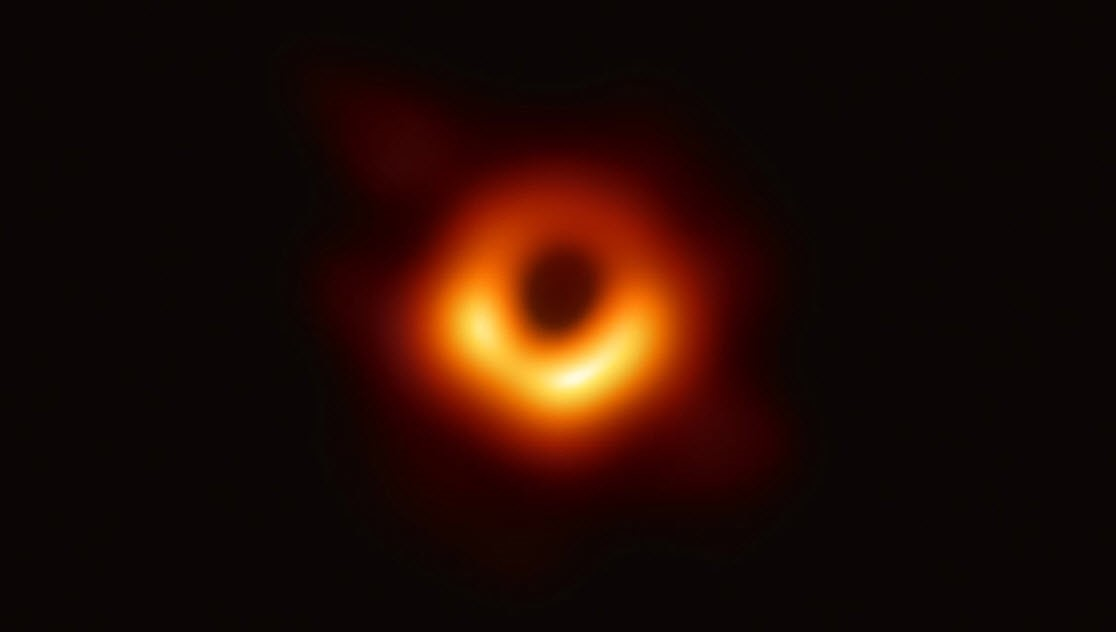
\includegraphics[width=3cm]{BlackHole}};
        \node[text=bg, font=\ttfamily] at ($(fig.center)!0.7!(fig.south)$) {/dev/null};
    \end{tikzpicture}
    \vspace{-9mm}
    \begin{columns}[c]
        \begin{column}{0.7\textwidth}
            \begin{varblock}{alerted}[\textwidth]{Do not be too clever!}<uncover@2>
                Suppressing the standard error might not be a so smart idea...
            \end{varblock}
        \end{column}
        \begin{column}{0.3\textwidth}
        \end{column}
    \end{columns}
    \bigskip
    \begin{lstlisting}[style=MyBash, numbers=none]
        $ echo 'Now you see me!'
        |+Now you see me!+|
        $ echo 'Now you do not see me!'  > /dev/null
        $ echo 'Now you do not see me!' >> /dev/null
        $ rm 'Who cares that this does not exists' 2>  /dev/null
        $ rm 'Who cares that this does not exists' 2>> /dev/null
    \end{lstlisting}
    \bigskip
    \begin{itemize}
        \item The file \texttt{/dev/null} is always empty, no matter what you write to it or read from it
        \item As such, when we write our (error) messages to it, they just disappear
        \item The \texttt{/dev/null} file remains as empty as ever before
        \item That's because it is not a normal file: It is a virtual device
        \item \PP{Redirecting \texttt{/dev/null} to \textbf{standard input} will give an immediate EOF to any read call}
    \end{itemize}
\end{frame}
%~~~~~~~~~~~~~~~~~~~~~~~~~~~~~~~~~~~~~~~~~~~~%
\begin{frame}[fragile]{Here Documents (I)}
    \vspace{-3mm}
    \begin{lstlisting}[style=MyBash, numbers=none]
        command |+[n]<<[-]WORD+|
            # here document
        |+WORD+|
    \end{lstlisting}
    \begin{itemize}
        \item Heredocs are useful to embed \textbf{short} blocks of multi-line data inside your script\\[-0.5ex]
              {\tiny\{~Embedding larger blocks is bad practice!~\}}
        \item In a Heredoc, you need to choose a \texttt{WORD} to act as a sentinel
        \item It can be any word: Choose one that won't appear in your data set
        \item All the lines that follow the first instance of the sentinel, up to the second instance, become the standard input for the \bash|command| 
        \item The second instance of the sentinel word has to be \alert{at the beginning of a line all by itself}
    \end{itemize}
    \begin{varblock}{quote}[0.7\textwidth]{Good practice}
        \textnormal{You should keep \PP{your logic} {\tiny\{~your code~\}} and \PP{your input} {\tiny\{~your data~\}} \PP{separated}, preferably in different files, unless it i    s a small data set!}
    \end{varblock}
\end{frame}
%~~~~~~~~~~~~~~~~~~~~~~~~~~~~~~~~~~~~~~~~~~~~%
\begin{frame}[fragile]{Here Documents (II)}
    \vspace{-5mm}
    \begin{enumerate}
        \item Standard form
              \begin{lstlisting}[style=MyBash, numbers=none, aboveskip=2mm, belowskip=-5mm]
                  command |+<<WORD+|
                      # here document subjected to parameter expansion,
                      # command substitution, and arithmetic expansion
                  |+WORD+|
              \end{lstlisting}
        \item Quoting (part of) the sentinel word
              \begin{lstlisting}[style=MyBash, numbers=none, aboveskip=2mm, belowskip=-5mm]
                  command <<'WORD'
                      # the lines in the here-document are not expanded
                  |+WORD+|
              \end{lstlisting}
        \item Adding a dash before the sentinel word to indent code
              \begin{lstlisting}[style=MyBash, numbers=none, aboveskip=2mm, belowskip=-5mm]
                  command |+<<-WORD+|
                      # Leading tabs (NOT spaces!) are removed
                  |+WORD+|
              \end{lstlisting}
        \item Combining the previous two forms is clearly allowed
    \end{enumerate}
    \FrameRemark{No parameter and variable expansion, command substitution, arithmetic expansion, or filename expansion is performed on \texttt{WORD}.}
\end{frame}
%~~~~~~~~~~~~~~~~~~~~~~~~~~~~~~~~~~~~~~~~~~~~%
\begin{frame}[fragile]{Here Documents (III): Examples}
    \vspace{-3mm}
    \begin{lstlisting}[style=MyBash]
        # Standard form
        $ if [[ $(date +'%A') |+!=+| S* ]]; then
        >     cat <<END
        >         Ouch, it is not weekend: $(date +'%A')
        > END
        > fi
        |+       Ouch, it is not weekend: Tuesday+|
        # Removing leading tabs
        $ cat <<-END
        >     abc seems to start with an a! # TAB before abc
        > END                               # (CTRL-v TAB)
        |+abc seems to start with an a!+|
        # Avoiding expansion
        $ cat <<-'SENTINEL'
        >     My home is ${HOME}            # TAB before My
        > SENTINEL
        |+My home is ${HOME}+|
    \end{lstlisting}
    \begin{uncoverenv}<2>
        \begin{lstlisting}[style=MyBash, numbers=none, aboveskip=4pt]
            cat |+<<EOF
            usage: foobar [-x] [-v] [-z] [file ...]
              A short explanation of the operation goes here.
              It might be few lines long, but should not be excessive.
            EOF+|
        \end{lstlisting}
    \end{uncoverenv}
\end{frame}
%~~~~~~~~~~~~~~~~~~~~~~~~~~~~~~~~~~~~~~~~~~~~%
\begin{frame}[fragile]{Here Strings}
    \vspace{-1mm}
    \begin{lstlisting}[style=MyBash, numbers=none]
        command |+[n]<<< STRING+|
    \end{lstlisting}
    \begin{itemize}[<only@1-2>]
        \item Herestrings are shorter, less intrusive and overall more convenient than Heredocs\\[-0.5ex]
              {\tiny\{~However, they are not portable to the Bourne shell~\}}
        \item The \texttt{STRING} undergoes:
              \begin{itemize}
                  \item tilde expansion
                  \item parameter and variable expansion
                  \item command substitution
                  \item arithmetic expansion
                  \item quote removal\tikzmark{quotes}
              \end{itemize}
        \item \alert{Pathname expansion} and word splitting \alert{are \textbf{not} performed}
        \item The result is supplied as a \alert{\textbf{single}} string, with a newline appended, to the \bash{command} on its standard input (or file descriptor \texttt{n} if specified)
    \end{itemize}
    \begin{varblock}{quote}[0.5\textwidth]{Good practice}<only@1-2>
        \textnormal{Prefer Herestrings to pipes whenever possible!}
    \end{varblock}
    \begin{onlyenv}<3>
        \begin{lstlisting}[style=MyBash, style=oddnumbers]
            $ grep |+--color=auto+| '[aeiou]' <<< "Clark Kent"
            @|Cl\tc{red}{a}rk K\tc{red}{e}nt|@
            $ bc <<< "10/4"
            |+2+|
            $ bc -l <<< "10/4"
            |+2.50000000000000000000+|
            $ bc <<< "obase=16; ibase=$(date +'%w'); 11000000"
            |+C0+|
            $ bc <<< "ibase=2; obase=10000; 11000000"
            |+C0+|
            $ wc -c <<< "Hello"
            |+6+|
            $ ls
            |+Day_1.pdf   Day_2.pdf+|
            $ echo *
            |+Day_1.pdf Day_2.pdf+|
            $ wc -c <<< *           # No filename expansion!
            |+2+|                       # Why 2 characters?
        \end{lstlisting}
    \end{onlyenv}
    \begin{tikzpicture}[remember picture, overlay, scope on=<2>]
        \path[from] (quotes) edge[out=0, in=270, looseness=0.5] node[pos=1, above, text=PT, draw=PQ, rounded corners=3mm, text width=30mm, align=center, font=\small] {Do not forget quotes, especially if the string contains spaces!} ++(5.2,1);
    \end{tikzpicture}
\end{frame}
%~~~~~~~~~~~~~~~~~~~~~~~~~~~~~~~~~~~~~~~~~~~~%
\againframe<3,5>{FDfigure}
%~~~~~~~~~~~~~~~~~~~~~~~~~~~~~~~~~~~~~~~~~~~~%
\begin{frame}[fragile]{Pipes}
    \vspace{-1mm}
    \begin{lstlisting}[style=MyBash, numbers=none]
        command | command
    \end{lstlisting}
    \begin{itemize}
        \item The pipe is created using the \PB{\texttt{|}} operator between two commands
        \item The former \bash{command}'s std output is connected to the latter \bash{command}'s std input
        \item This connection is performed before any redirection specified by the commands
        \item Pipes are widely used as a means of post-processing application output
        \item \alert{The pipe operator creates a subshell environment for each command!} \,{\tiny\{~More on subshells tomorrow~\}}
    \end{itemize}
    \begin{onlyenv}<1>
        \begin{lstlisting}[style=MyBash]
            $ message='Test'
            $ echo 'Salut, le monde!' | read message
            $ echo "The message is: $message"
            |+The message is: Test+|
            $ echo 'Salut, le monde!' | { read message;
            > echo "The message is: $message"; }
            |+The message is: Salut, le monde!+|
            $ echo "The message is: $message"
            |+The message is: Test+|
        \end{lstlisting}
    \end{onlyenv}
    \begin{onlyenv}<2>
        \begin{lstlisting}[style=MyBash, numbers=none]
            command 2>&1 |  command
            command      |& command
        \end{lstlisting}
        \begin{itemize}
            \item \PB{\texttt{|\&}} also connects the first \bash{command}'s std error to the second \bash{command}'s std input
            \item It is shorthand for \PB{\texttt{2>\&1 |}}
            \item This implicit redirection is performed after any redirection specified by the commands
        \end{itemize}
    \end{onlyenv}
\end{frame}
%~~~~~~~~~~~~~~~~~~~~~~~~~~~~~~~~~~~~~~~~~~~~%
\begin{frame}[fragile]{Pipes: A simple example}
    \vspace{-2mm}
    \begin{lstlisting}[style=MyBash]
        # Finding the maximum of a list
        $ for index in {1..5}; do
        >     echo $((RANDOM/RANDOM)).${RANDOM}
        > done
        |+1.4122
        2.15901
        0.19098
        0.6631
        0.15050+|
        $ for index in {1..5}; do
        >     echo $((RANDOM/RANDOM)).${RANDOM}
        > done | sort -n
        |+0.1455
        0.32373
        0.9598
        1.18896
        1.2768+|
        $ for index in {1..5}; do
        >     echo $((RANDOM/RANDOM)).${RANDOM}
        > done | sort -n | tail -n1
        |+2.21350+|
    \end{lstlisting}
\end{frame}
%~~~~~~~~~~~~~~~~~~~~~~~~~~~~~~~~~~~~~~~~~~~~%
\begin{frame}[fragile]{Pipes: Exit codes}
    \vspace{-3mm}
    \begin{itemize}
        \item The exit status of a pipeline is the exit status of the last command in the pipeline
        \item Bash provides an array variable \bash|PIPESTATUS| containing a list of exit status values from the processes in the most-recently-executed foreground process
    \end{itemize}
    \begin{lstlisting}[style=MyBash]
        $ for index in {1..5}; do
        >     echo $((RANDOM/RANDOM)).${RANDOM}
        > done | sort -n | tail -n1 | grep 'x'
        $ echo $?
        1
        $ for index in {1..5}; do
        >     echo $((RANDOM/RANDOM)).${RANDOM}
        > done | sort -n | tail -n1 | grep 'x'
        $ echo ${PIPESTATUS[@]}
        |+0 0 0 1+|
        $ for index in {1..5}; do
        >     echo $((RANDOM/RANDOM)).${RANDOM}
        > done | sort -n | rm 2> /dev/null | tail -n1 | grep 'x'
        $ echo ${PIPESTATUS[@]}
        |+0 141 1 0 1+| # @|\URL[red]{https://stackoverflow.com/a/19120674}{Pipes must have a reader (rm is not) and a writer}[background-color]|@
    \end{lstlisting}
    \FrameRemark{If \texttt{pipefail} is enabled, the pipeline's return status is the value of the rightmost command to exit with a non-zero status, or zero if all commands exit successfully.}
\end{frame}
%~~~~~~~~~~~~~~~~~~~~~~~~~~~~~~~~~~~~~~~~~~~~%
\begin{frame}[fragile]{Process substitution}
    \vspace{-3mm}
    \begin{lstlisting}[style=MyBash, numbers=none]
        command <(list)   # No space between < and (
        command >(list)   # No space between > and (
    \end{lstlisting}
    \vspace{3mm}
    \begin{onlyenv}<1>
        \begin{enumerate}\small
            \item The process list is run asynchronously, and its input or output appears as a filename
            \item This filename is passed as an argument to the current command as the result of the expansion\\[0.3em]
                  \begin{description}[\texttt{>(list)}]
                      \setlength{\itemsep}{2mm}
                      \item[\texttt{>(command\_list)}] ~\\[0.3em]
                          \hspace{-1cm}writing to the file will provide input for \PB{\texttt{command\_list}}\, {\tiny\{~Rarely needed!~\}}
                      \item[\texttt{<(command\_list)}] ~\\[0.3em]
                          \hspace{-1cm}the file passed as an argument should be read to obtain the output of \PB{\texttt{command\_list}}
                  \end{description}
        \end{enumerate}
        \begin{varblock}{}[0.82\textwidth]{The power of process substitution}
            Piping the stdout of a command into the stdin of another is a powerful technique.
            But, what if you need to pipe the stdout of multiple commands?\\
            \textbf{This is where process substitution comes in!}
        \end{varblock}
    \end{onlyenv}
    \begin{onlyenv}<2>
        \begin{lstlisting}[style=MyBash, xleftmargin=2mm, xrightmargin=0mm]
            $ cat <(date)   # Equivalent to a pipeline
            |+Wed 24 Jul 16:37:23 CEST 2019+|
            $ echo <(date)
            |+/dev/fd/63+|
            # Here a pipeline is not enough!
            $ cat <(date +'%T-%N') <(date +'%T-%N') <(date +'%T-%N')
            |+16:43:16-957108564+|
            |+16:43:16-958083851+|  # <(...) <(...) <(...) happen 'concurrently'@|$^\star$|@
            |+16:43:16-957603584+|
            $ echo <(date +'%T-%N') <(date +'%T-%N') <(date +'%T-%N')
            |+/dev/fd/63 /dev/fd/62 /dev/fd/61+|
            $ cat < <(date)
            |+Wed 24 Jul 16:53:43 CEST 2019+|
            $ echo < <(date)
            # Why do you get a blank output here?
            $ sdiff -s <(head Day_1.tex) <(head Day_2.tex)
            |+\subtitle{Day 1}                        | \subtitle{Day 2}
            \date{07.10.2019}                       | \date{08.10.2019}+|
        \end{lstlisting}
    \end{onlyenv}
    \FrameRemark[2]{$^\star$This is an incomplete statement, if taken as general rule: It is not \URL[PB]{https://unix.stackexchange.com/questions/403783/the-process-substitution-output-is-out-of-the-order}{the full story}.}
\end{frame}
%~~~~~~~~~~~~~~~~~~~~~~~~~~~~~~~~~~~~~~~~~~~~%

    \addSection{Compound commands}[0.45,0.09]{Skogafoss}{The Skogafoss cascade}
    %-------------------------------%
%  Author: Alessandro Sciarra   %
%    Date: 21 Aug 2019          %
%-------------------------------%

%~~~~~~~~~~~~~~~~~~~~~~~~~~~~~~~~~~~~~~~~~~~~%
\begin{frame}{Compound commands}
    \begin{itemize}
        \item \only<2>{\pgfsetfillopacity{0.5}}\bash{if} statements\tikzmark{doneStart}
        \item \bash{for} loops
        \item \bash{while}, \bash{until} loops
        \item \bash{[[} keyword
        \item \bash{case}, \bash{select} constructs\tikzmark{doneEnd}\pgfsetfillopacity{1}\medskip
        \item \tc<2>{PP}{Subshells}\tikzmark{nowStart}
        \item \tc<2>{PP}{Command grouping}
        \item \tc<2>{PP}{Arithmetic evaluation}\tikzmark{nowEnd}\\[-0.5ex] {\tiny\{~Slightly different from the \PQ{Arithmetic expansion} we already discussed~\}}\medskip
        \item \tc<2>{PB}{[Functions]\tikzmark{fcts}} {\tiny\{~Discussed in detail in a separate section~\}}
    \end{itemize}
    \begin{tikzpicture}[remember picture, overlay]
        \begin{scope}[scope on=<2>]
            \draw[very thick, decorate, decoration={brace,amplitude=6pt}] (doneStart -| doneEnd) ++(8mm,1mm) -- ($(doneEnd)+(8mm,-1mm)$) 
                      node[midway, right=3mm, text width=40mm, align=center] {Already discussed in details};
            \draw[very thick, decorate, decoration={brace,amplitude=6pt}, PP] (nowStart -| nowEnd) ++(8mm,1mm) -- ($(nowEnd)+(8mm,-1mm)$) 
                      node[midway, right=3mm, text width=40mm, align=center, text=PP] {What we are going to discuss};
            \path[from, PB] ($(fcts)-(6.8mm,3mm)$) edge[out=270, in=180] node[pos=1, right, font=\footnotesize, text=PB] {Strictly speaking not a compound command, but they work in a similar way} ++(2cm,-1cm);
        \end{scope}
    \end{tikzpicture}
\end{frame}
%~~~~~~~~~~~~~~~~~~~~~~~~~~~~~~~~~~~~~~~~~~~~%
\begin{frame}{Subshells}
    \vspace{-8mm}
    \begin{overlayarea}{\textwidth}{0.7\textheight}
        \begin{varblock}{}[0.8\textwidth]{Definition}
            A subshell is \textbf{a child process} but it is one \textbf{that inherits more than a normal external command} does.
            It can see all the variables of your script, not just the ones that have been exported to the environment.
        \end{varblock}
        \begin{varblock}{quote}[0.88\textwidth]{Unix Process}<only@1>
            Every process on a Unix system has its own parcel of memory, for holding its variables, its file descriptors, its copy of the Environment inherited from its parent process, and so on.
            The changes to the variables (and other private information) in one process do not affect any other processes currently running on the system.
        \end{varblock}
        \begin{varblock}{alerted}[0.6\textwidth]{Use them consciously}<only@1>
            Forking a subshell leads to a speed penalty which often is irrelevant but which you should keep in mind!
        \end{varblock}
        \begin{itemize}[<2>]
            \item It is explicitly forced using the parenthesis \PB{\texttt{(\ldots)}}
            \item Changes e.g. to variables done in a subshell are not remembered when exiting the subshell: A subshell can be thought as a temporary shell!
            \item There are many instances in which a shell creates a subshell without parentheses being placed by the programmer
                  \begin{itemize}
                      \item \PP{In pipelines} $\;\longleftarrow\;$ \alert{\textbf{Every command in a pipeline is run in its own subshell!}}
                      \item \PP{In command substitution}
                      \item Executing other programs or scripts
                      \item In any external command that executes new shells (e.g. \bash{awk}, \bash{sed}, \bash{perl})
                      \item In process substitution
                      \item In backgrounded commands and coprocs
                  \end{itemize}
        \end{itemize}
    \end{overlayarea}
    \FrameRemark[2]{From Bash v4.2 the shell option \texttt{lastpipe} can be enabled so that the last command in a pipeline is not run in a subshell.}
\end{frame}
%~~~~~~~~~~~~~~~~~~~~~~~~~~~~~~~~~~~~~~~~~~~~%
\begin{frame}[fragile]{Subshells: Examples}
    \begin{lstlisting}[style=MyBash]
        # Changes in a subshell do not propagate back
        $ aVar="Hello"; pwd
        /home/sciarra/Documents
        $ ( aVar="Goodbye"; echo "${aVar}" ); echo "${aVar}"
        |+Goodbye+|
        |+Hello+|
        $ ( cd /tmp; pwd ); pwd
        |+/tmp
        /home/sciarra/Documents+|
        # It is often a feature to take advantage of!
        $ (cd /tmp || exit 1; tar ...)
        $ (source ~/AuxiliaryBashTools.bash; ...)
        # In a subshell the script variable are accessible
        $ ( echo "${aVar} from the subshell" )
        |+Hello from the subshell+|
        # Implicit subshells: be aware of them!
        $ echo "Goodbye" | read aVar; echo "${aVar}"
        |+Hello+|
        $ read aVar <<< "Goodbye"; echo "${aVar}"; unset aVar
        |+Goodbye+|
    \end{lstlisting}
    \FrameRemark{\URL[PB]{http://mywiki.wooledge.org/BashFAQ/024}{Advanced reading} about pipelines and subshells: Why can't I pipe data to read?}
\end{frame}
%~~~~~~~~~~~~~~~~~~~~~~~~~~~~~~~~~~~~~~~~~~~~%
\begin{frame}[fragile]{Command grouping}{We already said something about it, let us go through once again}
    \vspace{-4mm}
    \begin{overlayarea}{\textwidth}{0.7\textheight}
        \begin{itemize}
            \item Commands may be grouped together using curly braces \PB{\texttt{\{\ldots\}}}
            \item Command groups allow a collection of commands to be considered as a whole with regards to redirection and control flow
            \item All compound commands such as \bash|if| statements and \bash|while| loops do this as well, but command groups do \textbf{only} this
            \item Command groups are executed in the same shell as everything else, NOT in a new one!
        \end{itemize}
        \begin{lstlisting}[style=MyBash, numbers=none]
            $ { echo "$(date)"
            >   rsync -av |+.+| /backup; echo "$(date)";@|\tikzmark{sc}|@ } >backup.log 2>&1
        \end{lstlisting}
        \smallskip
        \begin{varblock}{quote}[0.9\textwidth]{}<only@1>
            The above example truncates and opens the file backup.log on stdout, then points stderr at where stdout is currently pointing (backup.log), then runs each command with those redirections applied.
            The file descriptors remain open until all commands within the command group complete before they are automatically closed.
            This means backup.log is only opened a single time, not opened and closed for each command.
        \end{varblock}
        \begin{tikzpicture}[remember picture, overlay]
            \begin{scope}[scope on=<2->]
                \path[from, PT] ($(sc)-(0.9mm,1.5mm)$) edge[out=270, in=90] node[pos=1, below, font=\large, text=PT] (q) {Why is this semicolon absolutely \textbf{mandatory}?} ++(0cm,-1cm);
            \end{scope}
            \node[visible on=<3->, text width=5.6cm, align=center, below = 1mm of q, font=\scriptsize] {Because otherwise the closing curly bracket would be a argument of the final \mbox{command} in the group, \bash|echo| in this case};
        \end{tikzpicture}
    \end{overlayarea}
\end{frame}
%~~~~~~~~~~~~~~~~~~~~~~~~~~~~~~~~~~~~~~~~~~~~%
\begin{frame}[fragile]{Arithmetic evaluation: The \bash|let| builtin}
    \vspace{-4mm}
    \begin{itemize}
        \item Sometimes we want to do arithmetic instead of string operations
        \item One way to do so is to use the \bash|let| builtin
              \begin{lstlisting}[style=MyBash, style=oddnumbers, aboveskip=2mm, belowskip=-6mm]
                  $ aVar=4+5; echo "${aVar}"
                  |+4+5+|
                  $ let aVar=4+5; echo "${aVar}"; unset aVar
                  |+9+|
              \end{lstlisting}
        \item However, it requires quotes to use arithmetic operators $\quad${\tiny\{~\bash|help let|~\}}
              \begin{lstlisting}[style=MyBash, style=oddnumbers, aboveskip=2mm, belowskip=-6mm]
                  $ let aVar=2<3
                  |+bash: 3: No such file or directory+|
                  $ let aVar='2<3'; echo "${aVar}"; unset aVar
                  |+1+|
              \end{lstlisting}
        \item \bash|let| accepts more than one expression
              \begin{lstlisting}[style=MyBash, style=oddnumbers, aboveskip=2mm, belowskip=-6mm]
                  $ let aVar='2<3' bVar=3*7; echo "${aVar} ${bVar}"
                  |+1 21+|
                  $ unset aVar bVar
              \end{lstlisting}
        \item If the last expression evaluates to 0, \bash|let| returns 1; \bash|let| returns 0 otherwise.
    \end{itemize}
\end{frame}
%~~~~~~~~~~~~~~~~~~~~~~~~~~~~~~~~~~~~~~~~~~~~%
\begin{frame}[fragile]{Arithmetic evaluation: The command grouping \PB{\texttt{((\ldots))}}}
    \vspace{-4mm}
    \begin{overlayarea}{\textwidth}{0.7\textheight}
        \begin{itemize}
            \item<only@1> \PB{\texttt{(( expression ))}} $\;$is  equivalent to$\;$ \bash|let "expression"|
            \item<only@1> No quote is needed in it, since only arithmetic operations are there performed
            \item<only@1> However, only one expression can be evaluated (not bad for the exit code)
                  \begin{lstlisting}[style=MyBash, style=oddnumbers, aboveskip=2mm, belowskip=-6mm]
                      $ (( aVar=7*3**2 )); echo "${aVar}"
                      |+63+|
                      $ (( aVar=1+${aVar}/20 )); echo "${aVar}"; unset aVar
                      |+4+|        # '${}' not really needed@|$^\star$|@
                  \end{lstlisting}
            \item<only@1> Although not a compound command, the arithmetic substitution uses the same syntax
                  \begin{lstlisting}[style=MyBash, style=oddnumbers, aboveskip=2mm, belowskip=-6mm]
                      $ (( aVar=7*3**2 )); echo "${aVar}"
                      |+63+|
                      $ echo "aVar=$(( 7*3**2 ))"; unset aVar
                      |+63+|
                  \end{lstlisting}
            \item<only@1> Assignments in arithmetic substitution work but are confusing and should be avoided!
                  \begin{lstlisting}[style=MyBash, style=oddnumbers, aboveskip=2mm, belowskip=-6mm]
                      $ echo "_${bVar}_ $(( bVar=7*3**2 )) _${bVar}_"
                      |+__ 63 _63_+|
                  \end{lstlisting}
            \item<only@2> Arithmetic evaluation is very helpful in combination with conditionals
                  \begin{lstlisting}[style=MyBash, aboveskip=2mm, belowskip=-6mm]
                      $ ((aVar=(5+2)*3))
                      $ if ((aVar == 21)); then
                      >   echo 'Blackjack!'
                      > fi
                      |+Blackjack!+|
                  \end{lstlisting}
            \item<only@2> Because the inside of \PB{\texttt{((\ldots))}} is C-like, a variable (or expression) that \PP{evaluates to zero} will be considered \PP{false} for the purposes of the arithmetic evaluation.
                  Then, because the evaluation is false, it will \PP{exit with a status of 1}.
                  Likewise, if the expression inside \PB{\texttt{((\ldots))}} \PS{is non-zero}, it will be considered \PS{true}; and since the evaluation is true, it will \PS{exit with status 0}.
                  \begin{lstlisting}[style=MyBash, aboveskip=2mm, belowskip=-6mm]
                      $ flag=0  # no error
                      $ while read line; do
                      >   if [[ ${line}= *err* ]]; then flag=1; fi
                      > done < inputfile
                      $ if ((flag)); then echo 'Houston, we have a problem!'; fi
                  \end{lstlisting}
        \end{itemize}
    \end{overlayarea}
    \FrameRemark[1]{$^\star$Using the \texttt{\$\{\}} makes Bash use \bash|''| for uninitialised variables and might trigger errors (\texttt{0} is used for uninitialised variables referenced without \texttt{\$\{\}} syntax).}
\end{frame}
%~~~~~~~~~~~~~~~~~~~~~~~~~~~~~~~~~~~~~~~~~~~~%


    \addSection{Functions}[0.25,0.22]{Keifarvatn2}{The Keifarvatn lake}
    %-------------------------------%
%  Author: Alessandro Sciarra   %
%    Date: 25 Sep 2020          %
%-------------------------------%

%~~~~~~~~~~~~~~~~~~~~~~~~~~~~~~~~~~~~~~~~~~~~%
\begin{frame}{Functions, finally! Overview}
    \vspace{-4mm}
    \begin{itemize}
        \item Functions are the last basic Bash feature we'll learn
              \begin{itemize}
                  \item They give you an incredible opportunity to structure and increase readability of your script
                  \item They can be used to split large script across multiple files in an elegant way
                  \item \alert{Learn them well, for real!}
              \end{itemize}
        \item \PB{Functions are a tricky world!}
        \item They have several features that we might call \textbf{issues} if compared to other languages
        \item[\PT{$\bullet$}] Indeed, functions in Bash are not as powerful as we might expect
              \begin{itemize}
                  \item[\PT{$\to$}] Return value
                  \item[\PT{$\to$}] Reusability
                  \item[\PT{$\to$}] Scope
                  \item[\PT{$\to$}] I/O + \ldots
              \end{itemize}
              \begin{varblock}{quote}[0.9\textwidth]{}[Greg's Wiki]
                  Don't bite the newbie for not understanding all this. Shell functions are totally f\texttt{***}ed. \\[-1.3ex] ~
              \end{varblock}
    \end{itemize}
    \vspace{-4mm}
    \begin{varblock}{example}[1.03\textwidth]{\textbf{Do not be scared!}}
        Learn, understand and use functions for what they are, not for what you would like them to be!
    \end{varblock}
\end{frame}
%~~~~~~~~~~~~~~~~~~~~~~~~~~~~~~~~~~~~~~~~~~~~%
\begin{frame}[fragile]{Basic syntax}
    \vspace{-2mm}
    \begin{lstlisting}[style=MyBash, numbers=none]
        # POSIX compliant syntax
        NAME () |+COMPOUND-COMMAND [ REDIRECTIONS ]+|
        # Totally equivalent syntax (in Bash), but not POSIX
        function NAME |+[()] COMPOUND-COMMAND [ REDIRECTIONS ]+|
    \end{lstlisting}
    \vspace{1mm}
    \begin{description}[X]
        \setlength{\itemsep}{3mm}
        \item[\textbf{NAME:}] ~\\
            A \textbf{sane} function name should be an alphanumeric string, maybe containing underscore and not starting with a number.
            However, insane names are accepted in Bash and, in principle, names like \PB{\texttt{:}} or \PB{\texttt{[\}\{}} are allowed.
            But please, avoid them! Really!! \Remark{\URL[PB]{https://stackoverflow.com/a/44041384}{Exploring allowed names}}
        \item[\textbf{COMPOUND-COMMAND:}] ~\\
            The body of a function can be any compound command.
            \begin{itemize}
                \item \bash|{ list; }| \alert{$\;\longleftarrow\;$ Use this if you do not have a reason to use a different one}
                \item \bash|(list)| or \bash|((expression))| or \bash|[[ expression ]]|
            \end{itemize}
            %This is typically \bash|{ list; }|, but three other forms of compound commands are technically allowed: \bash|(list)|, \bash|((expression))|, and \bash|[[ expression ]]|.
        \item[\textbf{REDIRECTIONS:}] ~\\
            They take place when the function is called and they refer to the whole compound-command.
    \end{description}
\end{frame}
%~~~~~~~~~~~~~~~~~~~~~~~~~~~~~~~~~~~~~~~~~~~~%
\begin{frame}[fragile]{Functions: The most basic example}
    \vspace{-5mm}
    \begin{varblock}{example}[0.95\textwidth]{Just accomplish a \textbf{detached} task}
        Whenever a block of code can be executed as standalone, without needing either input information nor variables, it is straightforward to include it in a dedicated function
    \end{varblock}
    \begin{lstlisting}[style=MyBash, xrightmargin=1mm, xleftmargin=1mm]
        #!/bin/bash
        
        function CreateListOfFiles()
        {
            printf "#%19s %20s %15s %20s %20s %6s     %s\n" \
                   "user" "group" "permissions"               \
                   "size(KB)" "permissions" "type" "path"
            find "${PWD}" |+-printf+| "%20u %20g %15m %20k %20M %6y     %p\n"
        }
    \end{lstlisting}
    \begin{varblock}{}[0.9\textwidth]{Note}
        This will do absolutely nothing when run. This is because it has only been stored in memory, much like a variable, but it has not yet been called.
    \end{varblock}
    \begin{uncoverenv}<2>
        \begin{lstlisting}[style=MyBash, firstnumber=10, xrightmargin=1mm, xleftmargin=1mm]
            CreateListOfFiles
        \end{lstlisting}
    \end{uncoverenv}
\end{frame}
%~~~~~~~~~~~~~~~~~~~~~~~~~~~~~~~~~~~~~~~~~~~~%
\begin{frame}[fragile]{Variables in functions and their scopes}
    \vspace{-4mm}
    \begin{overlayarea}{\textwidth}{0.7\textheight}
        \begin{itemize}
            \item Variable in Bash are by definition \alert{\textbf{global}}!
            \item Variables declared using the \bash|local| builtin have a lifetime limited to the function scope
            \item Bash uses \textbf{dynamic scoping} to control a variable's visibility within functions
                  \begin{itemize}
                      \item In a function all variables visible in the caller are visible and might be changed
                      \item Declaring a local variable with the same name of an already existing variable shadows the variable from the caller, whose value cannot be retrieved from within the function.
                  \end{itemize}
            \item<only@3-> Unless you have a reason not to do so, declare all variables in functions as \bash|local|
            \item<only@3-> Do not assign a value to a local variable at declaration, because you might obfuscate/loose an exit code!
            \item<only@4-> \PP{If a variable at the current local scope is unset, it will remain so until it is reset in that scope or until the function returns.
                           Once the function returns, any instance of the variable at a previous scope will become visible.}\\
                           \textbf{However,} \PB{if the unset acts on a variable at a previous scope, any instance of a variable with that name that had been shadowed will become visible!}
        \end{itemize}
        \begin{onlyenv}<1>
            \begin{lstlisting}[style=MyBash]
                #!/bin/bash

                LevelOne() {
                    LevelTwo
                    echo "In ${FUNCNAME}, aVar = ${aVar}"
                }
                LevelTwo() {
                    local aVar; aVar="${FUNCNAME} local"
                    LevelThree
                }
                LevelThree() { echo "In ${FUNCNAME}, aVar = ${aVar}"; }

                aVar='global'; LevelOne
            \end{lstlisting}
        \end{onlyenv}
        \begin{onlyenv}<2>
            \begin{lstlisting}[style=MyBash, firstnumber=14]
                $ ./script.bash
                |+In LevelThree, aVar = LevelTwo local
                In LevelOne, aVar = global+|
            \end{lstlisting}
        \end{onlyenv}
        \begin{onlyenv}<3>
            \begin{lstlisting}[style=MyBash, style=oddnumbers, xleftmargin=1mm, xrightmargin=1mm, firstnumber=16]
                $ function Test { aVar="$(exit 1)"; echo $?; }; Test
                1  # Fine, but we pollute caller with 'aVar' variable
                $ function Test { local aVar="$(exit 1)"; echo $?; }; Test
                0  # <- local's exit code!
                $ function Test { local aVar; aVar="$(exit 1)"; echo $?; }; Test
                1  # GOOD CODE
            \end{lstlisting}
        \end{onlyenv}
    \end{overlayarea}
\end{frame}
%~~~~~~~~~~~~~~~~~~~~~~~~~~~~~~~~~~~~~~~~~~~~%
\begin{frame}{Passing arguments to functions}
    \vspace{-3mm}
    \begin{varblock}{example}[0.8\textwidth]{So far so good}
        Delegating tasks to functions, even if the task requires variables, is quite straightforward, provided one keeps scope rules in mind
    \end{varblock}
    \begin{varblock}{quote}[0.95\textwidth]{The Pandora's box}[Bash manual]<2->
        When a function is executed, the arguments to the function become the positional parameters during its execution.
        The special parameter \texttt{\#} that expands to the number of positional parameters is updated to reflect the change.
        Special parameter 0 is unchanged.\\[-1.5ex] ~
    \end{varblock}
    \vspace{-2mm}
    \begin{itemize}[<3->]
        \item Arguments to functions are meant to provide \textbf{input} to a function
        \item Bash strictly uses \PP{call-by-value} semantics
        \item You can't pass arguments ``by reference''\\[-0.5ex] \Remark{at least not until Bash 4.3 (and even there the \bash|declare -n| mechanism has serious security flaws)}
        \item \alert{Passing the name of a variable to a function}, which should use it, requires \bash|eval| acrobatics and it \alert{should be as far as possible avoided!}
    \end{itemize}
\end{frame}
%~~~~~~~~~~~~~~~~~~~~~~~~~~~~~~~~~~~~~~~~~~~~%
\begin{frame}[fragile]{Passing arguments to functions: Example}
    \vspace{-2mm}
    \begin{onlyenv}<1>
        \begin{lstlisting}[style=MyBash]
            #!/bin/bash

            function SecondsToTimeStringWithDays()
            {
                local inputTime days hours minutes seconds
                inputTime=$1
                ((    days=(inputTime)/86400 ))
                ((   hours=(inputTime - days*86400)/3600 ))
                (( minutes=(inputTime - days*86400 - hours*3600)/60 ))
                (( seconds=inputTime%60 ))
                printf "%d-%02d:%02d:%02d\n" \
                       "${days}" "${hours}" "${minutes}" "${seconds}"
            }

            for example in 31536000 86400 3600; do
                SecondsToTimeStringWithDays ${example}
            done
        \end{lstlisting}
        \begin{lstlisting}[style=MyBash, aboveskip=2mm, firstnumber=18]
            $ ./scriptAbove
            |+365-00:00:00+|
            |+1-00:00:00+|     # What is bad in the function above?
            |+0-01:00:00+|
        \end{lstlisting}
    \end{onlyenv}
    \begin{onlyenv}<2>
        \begin{lstlisting}[style=MyBash, firstnumber=22]
            #!/bin/bash

            function SecondsToTimeStringWithDays() # Better code!
            {
                if [[ ! ${1} =~ ^[1-9][0-9]*$ ]]; then
                   echo "ERROR: Function ${FUNCNAME} wrongly called!"
                   return 1
                fi
                local inputTime days hours minutes seconds
                inputTime=$1
                ((    days=(inputTime)/86400 ))
                ((   hours=(inputTime - days*86400)/3600 ))
                (( minutes=(inputTime - days*86400 - hours*3600)/60 ))
                (( seconds=inputTime%60 ))
                printf "%d-%02d:%02d:%02d\n" \
                       "${days}" "${hours}" "${minutes}" "${seconds}"
            }

            for example in 31536000 86400 3600 ''; do
                SecondsToTimeStringWithDays ${example}
            done
        \end{lstlisting}
    \end{onlyenv}
\end{frame}
%~~~~~~~~~~~~~~~~~~~~~~~~~~~~~~~~~~~~~~~~~~~~%
\begin{frame}[fragile]{The \bash|return| builtin and functions' exit code}
    \vspace{-4mm}
    \begin{varblock}{quote}[0.6\textwidth]{Functions' exit code}
        \textnormal{When executed, the exit status of a function is the exit status of the \textbf{last command executed} in the body.}
    \end{varblock}
    \begin{lstlisting}[style=MyBash, numbers=none, belowskip=-6mm]
        $ help return
        |+return: return [n]+|           # ATTENTION: 0 <= N <=255
        |+Return from a shell function.

        Causes a function or sourced script to exit with the
        return value specified by N. If N is omitted, the
        return status is that of the last command executed
        within the function or script.

        Exit Status:
        Returns N, or failure if the shell is not executing
        a function or script.+|
    \end{lstlisting}
    \medskip
    \begin{varblock}{alert}[0.65\textwidth]{}
        \large \alert{Do not use \bash|return| to retrieve the function result!}
    \end{varblock}
    \vspace{-1mm}
    \begin{varblock}{example}[0.85\textwidth]{}
        \PS{Use \bash|return| to early terminate a function and/or to give back an exit code!}
    \end{varblock}
\end{frame}
%~~~~~~~~~~~~~~~~~~~~~~~~~~~~~~~~~~~~~~~~~~~~%
\begin{frame}[fragile]{How do I return something from a function?}
    \vspace{-18.2mm}
    \begin{overlayarea}{\textwidth}{0.7\textheight}
        \begin{columns}[c]
            \begin{column}{0.55\textwidth}
            \end{column}
            \begin{column}{0.35\textwidth}
                \begin{varblock}{alert}[\textwidth]{}<2->
                    \Large It's simple: \alert{You don't!}
                \end{varblock}
            \end{column}
        \end{columns}
        \smallskip
        \setbeamertemplate{itemize/enumerate subbody begin}{\scriptsize}
        \begin{enumerate}
            \item<only@3-> Capturing standard output
                           \begin{itemize}[<only@{3,7}>]
                               \item[\crossmark] the function is executed in a subshell, i.e. variable assignments not seen in the caller
                               \item[\crossmark] \textbf{everything} printed by the function is captured (debug output!? $\to$ use stderr)
                               \item[\checkmark] good solution if performance is not critical
                           \end{itemize}
            \item<only@4-> Global variables
                           \begin{itemize}[<only@{4,7}>]
                               \item[\checkmark] the function is \textbf{not} executed in a subshell $\to$ potentially \PS{much faster}
                               \item[\crossmark] if the function is executed in a subshell, the method fails!
                               \item[\crossmark] the function cannot be used in a pipeline (as in any implicit subshell)
                           \end{itemize}
            \item<only@5-> Writing to a file
                           \begin{itemize}[<only@{5,7}>]
                               \item[\crossmark] you need to manage a temporary file, which is always inconvenient
                               \item[\crossmark] there must be a writable directory somewhere and sufficient space to hold the data therein
                               \item[\checkmark] it will work regardless of whether your function is executed in a subshell
                           \end{itemize}
            \item<only@6-> Dynamically scoped variables
                           \begin{itemize}
                               \item[\crossmark] if the function is executed in a subshell, the method fails!
                               \item[\crossmark] this technique doesn't work with recursive functions
                               \item[\checkmark] global variable namespace isn't polluted by the function return variable
                           \end{itemize}
        \end{enumerate}
        \begin{onlyenv}<3>
            \begin{lstlisting}[style=MyBash, numbers=none]
                ExampleFunction() {
                    echo "running foo()..."  >&2
                    echo "this is my data"
                }
                aVar=$(ExampleFunction)
                echo "ExampleFunction returned '${aVar}'"
            \end{lstlisting}
        \end{onlyenv}
        \begin{onlyenv}<4>
            \begin{lstlisting}[style=MyBash, numbers=none]
                ExampleFunction() {
                    globalVar="this is my data"
                }
                ExampleFunction
                echo "ExampleFunction returned '${globalVar}'"
            \end{lstlisting}
        \end{onlyenv}
        \begin{onlyenv}<5>
            \begin{lstlisting}[style=MyBash, numbers=none]
                ExampleFunction() {
                    echo "this is my data" > "$1"
                }
                # This is NOT solid code to handle temp files! @|\URL[comment-color]{http://mywiki.wooledge.org/BashFAQ/062}{Solid way}[background-color]|@
                tmpfile=$(mktemp)   # GNU/Linux
                ExampleFunction "${tmpfile}"
                echo "ExampleFunction returned '$(cat < "@|\tc{strings-color}{\$\{tmpfile\}}|@" )'"
                rm "${tmpfile}"
            \end{lstlisting}
            \FrameRemark[5]{If this were a real program, there would have been error checking, and a trap.}
        \end{onlyenv}
        \begin{onlyenv}<6>
            \begin{lstlisting}[style=MyBash, numbers=none, emph={[7]notGlobalVar},]
                ExampleFunction_implementation() {
                   notGlobalVar="this is my data"
                }
                ExampleFunction() {
                    local notGlobalVar; ExampleFunction_implementation
                    # Do here something with 'notGlobalVar'
                    echo "In ExampleFunction, got '${notGlobalVar}'"
                }
                # Here at the global scope, 'notGlobalVar' is not visible
                ExampleFunction
                echo "ExampleFunction returned '${notGlobalVar}'"
            \end{lstlisting}
        \end{onlyenv}
        \vspace{-3mm}
        \begin{varblock}{}[0.7\textwidth]{Choose with care}<only@7>
            Use the approach you prefer depending on the situation!
        \end{varblock}
    \end{overlayarea}
\end{frame}
%~~~~~~~~~~~~~~~~~~~~~~~~~~~~~~~~~~~~~~~~~~~~%
\begin{frame}[fragile]{Splitting large scripts across multiple files}{A Bash script should not be \textbf{too} large, though}
    \vspace{-3mm}
    \begin{onlyenv}<1>
        \begin{varblock}{example}[0.9\textwidth]{Declaring a function does not mean to run it}
            You can collect functions in a separate file, which is meant to be sourced at need!
        \end{varblock}
        \begin{lstlisting}[style=MyBash, numbers=none]
            # Collection of tools

            function ExtractColumnFromFile()
            {
                # ...
            }

            function CalculateSizeOfFiles()
            {
                # ...
            }

            function ReportOnLargestDirectories()
            {
                # ...
            }
        \end{lstlisting}
    \end{onlyenv}
    \begin{onlyenv}<2>
        \begin{lstlisting}[style=MyBash, numbers=none]
            #!/bin/bash

            source /home/sciarra/Script/UtilityFunctions.bash
            source /home/sciarra/Script/UtilityFunctions_nice.bash
            source /home/sciarra/Script/UtilityFunctions_cool.bash

            # Call to functions (only, maybe)
        \end{lstlisting}
        \begin{itemize}
            \item \PP{As long as the sourced files contain functions only},
                  \begin{itemize}
                      \item the \textbf{sourcing order does not matter} and
                      \item functions in a file can even use functions in another file!
                  \end{itemize}
            \item The shebang can/should be included in the main file only!
            \item Prevent auxiliary files from being run, only sourced!
        \end{itemize}
        \begin{lstlisting}[style=MyBash, numbers=none, xleftmargin=1mm, xrightmargin=1mm]
            if [[ "${BASH_SOURCE[0]}" == "${0}" ]]; then
              echo "Script \"${BASH_SOURCE[0]}\" can only been sourced!" 2>&1
              exit -1
            fi
        \end{lstlisting}
    \end{onlyenv}
\end{frame}
%~~~~~~~~~~~~~~~~~~~~~~~~~~~~~~~~~~~~~~~~~~~~%
\begin{frame}[fragile]{Functions: Miscellaneous}
    \begin{overlayarea}{\textwidth}{0.7\textheight}
        \begin{onlyenv}<1>
            \vspace{-3mm}
            \begin{itemize}
                \item Functions can be marked as read-only using the \bash|readonly| builtin
                \item Functions can be unset via \,\bash|unset -f|
                \item Functions can be recursive
                      \begin{lstlisting}[style=MyBash, xrightmargin=12mm, aboveskip=2mm, belowskip=-6mm]
                          function CountTill5From()
                          {
                              if [[ $1 < 5 ]]; then
                                  echo $1; CountTill5From $(($1 + 1))
                              fi
                          }
                      \end{lstlisting}
                \item The \bash|FUNCNEST| variable may be used to limit the depth of the function call stack and restrict the number of function invocations
                      \Remark{By default, no limit is placed on the number of recursive calls}
            \end{itemize}
            \begin{lstlisting}[style=MyBash, xrightmargin=-2mm, xleftmargin=2mm, aboveskip=0mm, numbers=none]
                $ FUNCNEST=2; CountTill5From()
                |+1
                2
                bash: CountTill5From: maximum function nesting level exceeded (2)+|
                $ unset -v FUNCNEST
            \end{lstlisting}
        \end{onlyenv}
        \begin{onlyenv}<2->
            \vspace{-9mm}
            \begin{varblock}{alert}[0.9\textwidth]{About recursion}
                \begin{itemize}
                    \item \emph{\guillemotleft To iterate is human, to recur, divine.\guillemotright} -- L. Peter Deutsch
                    \item There are cases where it is needed
                    \item In Bash rarely, though
                    \item The fact that by default in Bash there is no limit to the number of function invocations is something to have clear in mind!
                    \item For example, what does the following code do? \,\alert{\textbf{DON'T RUN IT!}}
                          \begin{lstlisting}[style=MyBash, numbers=none, aboveskip=2mm, belowskip=-6mm, xrightmargin=21mm]
                              :(){ :|:& };:   # Do NOT run this line!
                          \end{lstlisting}
                          \begin{uncoverenv}<3>
                              It is equivalent to
                              \begin{lstlisting}[style=MyBash, numbers=none, aboveskip=2mm, belowskip=-5mm, xrightmargin=21mm]
                                  # Do NOT run this code!
                                  function bomb() { bomb | bomb & }; bomb
                              \end{lstlisting}
                          \end{uncoverenv}
                \end{itemize}
            \end{varblock}
            \vspace{-1mm}
            \begin{varblock}{quote}[\textwidth]{}[Wikipedia]<only@3>
                \small A \textbf{fork bomb} is a denial-of-service attack wherein a process continually replicates itself to deplete available system resources,
                \textbf{slowing down or crashing the system} due to resource starvation.\\[-1.5ex] ~
            \end{varblock}
        \end{onlyenv}
    \end{overlayarea}
\end{frame}
%~~~~~~~~~~~~~~~~~~~~~~~~~~~~~~~~~~~~~~~~~~~~%
\begin{frame}[fragile]{A last big warning: The \bash|eval| builtin}
    \vspace{-3mm}
    \begin{overlayarea}{\textwidth}{0.64\textheight}
        \begin{onlyenv}<1>
            \begin{lstlisting}[style=MyBash, numbers=none, xleftmargin=2mm, xrightmargin=2mm]
                $ help eval
                |+eval: eval [arg ...]
                Execute arguments as a shell command.

                Combine ARGs into a single string, use the result as input
                to the shell, and execute the resulting commands.

                Exit Status:
                Returns exit status of command or success if command is null.+|
            \end{lstlisting}
            \begin{itemize}
                \item \emph{\guillemotleft\textnormal{\bash|eval|} is a common misspelling of \textbf{evil}\guillemotright} -- Greg's Wiki
                \item It causes your code to be parsed twice instead of once; this means that, for example, if your code has variable references in it, the shell's parser will evaluate the contents of that variable.
                      This can lead to unexpected results!
            \end{itemize}
        \end{onlyenv}
        \begin{onlyenv}<2->
            \begin{lstlisting}[style=MyBash, emph={[7]_fifth_array}]
                # This code is evil and should never be used!
                function FifthElementOf() {
                  local _fifth_array=$1
                  eval echo "\"The fifth element is \${$_fifth_array[4]}\""
                }
            \end{lstlisting}
            \smallskip
            \begin{lstlisting}[style=MyBash, emph={[7]_fifth_array}, belowskip=-5mm, firstnumber=6]
                # Source/define the function above
                $ array=(zero one two three four five)
                $ FifthElementOf array
                |+The fifth element is four+|
            \end{lstlisting}
            You might be thinking -- \PP{``It looks OK, isn't it? What's wrong man?''} \uncover<3->{-- Consider then:}
        \end{onlyenv}
        \begin{onlyenv}<3>
            \begin{lstlisting}[style=MyBash, emph={[7]_fifth_array}, aboveskip=2mm, firstnumber=10]
                $ FifthElementOf 'x}"; da@|\tikzmark{date}|@te; #'
            \end{lstlisting}
        \end{onlyenv}
        \begin{onlyenv}<4->
            \begin{lstlisting}[style=MyBash, emph={[7]_fifth_array}, aboveskip=2mm, firstnumber=10]
                $ FifthElementOf 'x}"; da@|\tikzmark{date}|@te; #'
                |+The fifth element is
                Wed 28 Aug 14:43:59 CEST 2019+|  # AAAAAARRRGGGGHHH!!!!
            \end{lstlisting}
        \end{onlyenv}
    \end{overlayarea}
    {\Large\begin{varblock}{alert}[\textwidth]{Take-home lesson}<4->
        An inappropriate use of \bash|eval| can lead to \alert{arbitrary code execution}!
    \end{varblock}}
    \begin{tikzpicture}[remember picture, overlay, scope on=<5>]
        \path[from] (date) edge[out=270, in=180] node[pos=1, right] {\color{red}What about $\;$ \bash|rm -rf /| $\;$ here?} ++(15mm,-1mm);
    \end{tikzpicture}
    \FrameRemark{Advanced, but \URL[PB]{http://mywiki.wooledge.org/BashFAQ/048}{very informative article} which you should spend some time at some point on.}
\end{frame}







    \addSection{Built in VS external programs}[0.735,0.255]{JokursarlonBeach4}{The volcanic beach of the J\"okurs\'arl\'on}
    %-------------------------------%
%  Author: Alessandro Sciarra   %
%    Date: 28 Aug 2019          %
%-------------------------------%

%~~~~~~~~~~~~~~~~~~~~~~~~~~~~~~~~~~~~~~~~~~~~%
\begin{frame}{Do not underestimate the difference}
    \vspace{-3mm}
    \begin{description}[XXX]
        \item[\textbf{Internal Commands:}] ~ \\
            Commands which are built into the shell.
            This means that the code that implements a builtin is in \bash|/bin/bash|.
        \item[\textbf{External Commands:}] ~ \\
            When an external command has to be executed, the shell looks for its path given in \bash|PATH| variable and also a new process has to be spawned and the command gets executed.
    \end{description}
    \begin{varblock}{example}[0.8\textwidth]{The precedence order for command names}
        \begin{enumerate}
            \item Alias
            \item Function {\tiny\{~You can shadow builtin commands creating a function with the same name~\}}
            \item Builtin  {\tiny\{~The \bash|builtin| builtin serves to refer to a shadowed builtin $\;\to\;$ \bash|help builtin|~\}}
            \item Keywords
            \item External command in the directories listed in \texttt{\$\{PATH\}} in order.
        \end{enumerate}
    \end{varblock}
\end{frame}
%~~~~~~~~~~~~~~~~~~~~~~~~~~~~~~~~~~~~~~~~~~~~%
\begin{frame}[fragile]{A trivial benchmark}
    \begin{lstlisting}[style=MyBash]
        $ mkdir tmpFolder; cd tmpFolder
        $ time for i in {1000..9999}; do echo > $i; done; echo
        |+
        real    0m12.026s
        user    0m0.434s
        sys     0m0.857s
        +|
        $ time for i in {1000..9999}; do /bin/echo > $i; done; echo
        |+
        real    0m27.441s
        user    0m9.504s
        sys     0m5.034s
        +|
        $ cd ..; rm -r tmpFolder
    \end{lstlisting}
    \medskip
    \begin{varblock}{}[0.9\textwidth]{Do not overdo, just keep it in mind}
        \begin{itemize}
            \item \emph{\guillemotleft Premature optimisation is the root of all evil\guillemotright} -- Donald Knuth
            \item Unnecessary use of external commands are welcome
        \end{itemize}
    \end{varblock}
\end{frame}
%~~~~~~~~~~~~~~~~~~~~~~~~~~~~~~~~~~~~~~~~~~~~%

    \addSection{Script autocompletion}[0.735,0.255]{DragonIceberg}{A ice-dragon on the J\"okurs\'arl\'on's beach}
    %-------------------------------%
%  Author: Alessandro Sciarra   %
%    Date: 25 Sep 2020          %
%-------------------------------%

%~~~~~~~~~~~~~~~~~~~~~~~~~~~~~~~~~~~~~~~~~~~~%
\begin{frame}[fragile]{Programmable completion}{A complex world plenty of opportunities: \enspace\URL[PB]{https://www.gnu.org/software/bash/manual/}{Bash manual v5.0 sections 8.6 and 8.7}}
    \vspace{-3mm}
    \begin{itemize}
        \item Whenever you press \texttt{TAB} while typing in your terminal,\\ \PS{you trigger a series of operations that the shell executes underneath}.
        \item This mechanism is actually programmable and it is usually available system-wide.
        \item It is nothing but\ldots\ a bash script to be sourced in your environment!
        \item It is usually automatically sourced somewhere, at university in the shell configuration file.
    \end{itemize}
    \begin{lstlisting}[style=myBash, numbers=none, aboveskip=2mm]
        # In a default ~/.bashrc file at some point:
        if [ -f /etc/bash_completion ]; then
            . /etc/bash_completion
        fi
    \end{lstlisting}
    \begin{lstlisting}[style=myBash, numbers=none, aboveskip=2mm, belowskip=-5mm]
        $ cat /etc/bash_completion
        |+. /usr/share/bash-completion/bash_completion+|
        $ wc -l /usr/share/bash-completion/bash_completion
        |+2171+|
    \end{lstlisting}
    \begin{itemize}
        \item The mechanism is triggered via the \bash|complete| builtin.
    \end{itemize}
\end{frame}
%~~~~~~~~~~~~~~~~~~~~~~~~~~~~~~~~~~~~~~~~~~~~%
\begin{frame}{The program completion ingredients}
    \vspace{-6mm}
    \begin{columns}
        \begin{column}{\dimexpr\paperwidth-18mm}
            \begin{onlyenv}<1>
                \begin{description}[\texttt{XXCOMP\_WORDS}]
                    \setlength{\itemsep}{2mm}
                    \item[\PB{\texttt{compgen}}]
                        Generate possible completion matches for word according to the options and write the matches to the standard output.
                    \item[\PB{\texttt{complete}}]
                        Specify how arguments should be completed.
                    \item[\PB{\texttt{compopt}}]
                        Modify completion options for each name according to the options, or for the currently-executing completion if no names are supplied.\\[6mm]
                    \item[\PB{\texttt{COMP\_WORDS}}]
                        An array variable consisting of the individual words in the current command line.
                    \item[\PB{\texttt{COMP\_CWORD}}]
                        An index into \PB{\texttt{\$\{COMP\_WORDS\}}} of the word containing the current cursor position.
                    \item[\PB{\texttt{COMPREPLY}}]
                        An array variable from which Bash reads the possible completions generated. Each array element contains one possible completion.
                \end{description}
            \end{onlyenv}
        \end{column}
    \end{columns}
    \FrameRemark{There are further relevant variables --- \bash|COMP_WORDBREAKS|, \bash|COMP_LINE|, \bash|COMP_POINT|, etc. --- refer to the \URL[PB]{https://www.gnu.org/software/bash/manual/}{Bash manual v5.0 sections 5.2}.}
\end{frame}
%~~~~~~~~~~~~~~~~~~~~~~~~~~~~~~~~~~~~~~~~~~~~%
\begin{frame}[fragile]{The standard pattern}
    \vspace{-3mm}
    \begin{enumerate}
        \item Make the script for which you want to implement autocompletion executable.
        \item Create an autocompletion script \textbf{to be sourced} in your environment.
        \item Associate a function to the command you want (your script's name) using.
              \begin{lstlisting}[style=myBash, numbers=none, aboveskip=3mm, belowskip=-5mm, xrightmargin=15mm]
                  complete -F _script_completion  script
              \end{lstlisting}
              After having sourced the autocompletion script, this function will be automatically invoked by the shell when pressing \texttt{TAB} after the name of your script.
        \item Write the autocompletion function keeping in mind how it works.
    \end{enumerate}
    \begin{varblock}{alert}[0.9\textwidth]{A standard invocation}
        \begin{itemize}
            \item \PB{\texttt{\$1}} is the name of the command whose arguments are being completed;
            \item \PB{\texttt{\$2}} is the word being completed;
            \item \PB{\texttt{\$3}} is the word preceding the word being completed;
            \item The array variable \PB{\texttt{COMPREPLY}} contains possible completions.
        \end{itemize}
    \end{varblock}
\end{frame}
%~~~~~~~~~~~~~~~~~~~~~~~~~~~~~~~~~~~~~~~~~~~~%
\begin{frame}[fragile]{A basic example as starting point}
    \vspace{-1mm}
    \begin{onlyenv}<1-2,8->
        Suppose to have a \,\PS{\texttt{measure}}\, script that accepts the following options on the command line:
        \begin{itemize}
            \item \PB{\texttt{-{}-inputfile}} followed by a filename;
            \item a series of other options, e.g. \PB{\texttt{-{}-verbose}} and \PB{\texttt{-{}-conservative}}.
        \end{itemize}
        How do I implement autocompletion for it?
        \begin{onlyenv}<2>
            \begin{lstlisting}[style=myBash, numbers=none, aboveskip=4mm]
                $ emacs -nw ~/.measure-completion.bash
            \end{lstlisting}
        \end{onlyenv}
    \end{onlyenv}
    \begin{onlyenv}<3>
        \begin{lstlisting}[style=myBash, numbers=none, style=smaller]
            #!/usr/bin/env bash
        \end{lstlisting}
    \end{onlyenv}
    \begin{onlyenv}<4>
        \begin{lstlisting}[style=myBash, numbers=none, style=smaller]
            #!/usr/bin/env bash

            if [[ "${BASH_SOURCE[0]}" = "${0}" ]]; then
                printf "\n ERROR: File \"${BASH_SOURCE[0]}\" cannot be executed!\n\n"
                exit 1
            fi
        \end{lstlisting}
    \end{onlyenv}
    \begin{onlyenv}<5-6>
        \begin{lstlisting}[style=myBash, numbers=none, style=smaller]
            #!/usr/bin/env bash

            if [[ "${BASH_SOURCE[0]}" = "${0}" ]]; then
                printf "\n ERROR: File \"${BASH_SOURCE[0]}\" cannot be executed!\n\n"
                exit 1
            fi

            function _measure_completion() @|\tikzmark{bad}|@
            {
                case "$3" in
                    --inputfile )
                        COMPREPLY=( $(compgen -f -- "$2") )
                        ;;
                    * )
                        COMPREPLY=(
                            $(compgen -W "--inputfile --verbose --conservative" -- "$2")
                        )
                        ;;
                esac
            }

            complete -F _measure_completion   measure
        \end{lstlisting}
    \end{onlyenv}
    \begin{onlyenv}<7>
            \begin{lstlisting}[style=myBash, numbers=none, style=smaller]
            #!/usr/bin/env bash

            if [[ "${BASH_SOURCE[0]}" = "${0}" ]]; then
                printf "\n ERROR: File \"${BASH_SOURCE[0]}\" cannot be executed!\n\n"
                exit 1
            fi

            function _measure_completion() @|\tikzmark{stillbad}|@
            {
                case "$3" in
                    --inputfile )
                        COMPREPLY=( $(compgen -f -- "$2") )
                        ;;
                    * )
                        COMPREPLY=(
                            $(compgen -W "--inputfile --verbose --conservative" -- "$2")
                        )
                        ;;
                esac
            }

            #complete -F _measure_completion   measure
            complete -o filenames -F _measure_completion   measure
        \end{lstlisting}
    \end{onlyenv}
    \begin{tikzpicture}[remember picture, overlay]
        \node[visible on=<6>, anchor=west, text=red, font=\small] at ($(bad)+(5mm,0)$) {What is bad in this implementation?};
        \node[visible on=<7>, anchor=west, text=red, font=\small] at ($(stillbad)+(5mm,0)$) {What is still bad in this implementation?};
    \end{tikzpicture}
    \begin{onlyenv}<8>
        \begin{lstlisting}[style=myBash, numbers=none, aboveskip=4mm]
            $ emacs -nw ~/.measure-completion.bash
            $ . ~/.measure-completion.bash
            $ ls
            file01.dat   file02.dat   file03.dat   @|\tc{RoyalBlue}{backup}|@
            $ ./measure <TAB>
            $ ./measure --<TAB-TAB>
            --conservative  --inputfile     --verbose
            $ ./measure --inputfile <TAB-TAB>
            backup/   file01.dat   file02.dat   file03.dat
            # There is room for improvement!
            $ ./measure --inputfile file02.dat <TAB-TAB>
            --conservative  --inputfile     --verbose
        \end{lstlisting}
    \end{onlyenv}
    \FrameRemark{Usually, you want to implement autocompletion for a script that you use very often. It is common to make it executable and remove the \,\texttt{.bash}\, extension.}
\end{frame}
%~~~~~~~~~~~~~~~~~~~~~~~~~~~~~~~~~~~~~~~~~~~~%

    \addSection{GNU Readline}[0.255,0.24]{RedRoad}{A trail at sunset in the Reykjanesf\'olkvangur Reserve}
    %-------------------------------%
%  Author: Alessandro Sciarra   %
%    Date: 28 Sep 2020          %
%-------------------------------%

%~~~~~~~~~~~~~~~~~~~~~~~~~~~~~~~~~~~~~~~~~~~~%
\begin{frame}{The GNU Readline Library}{\URL[PB]{https://tiswww.case.edu/php/chet/readline/rltop.html}{Official website}}
    \vspace{-3mm}
    \begin{varblock}{}[0.9\textwidth]{What is it for?}
        The GNU Readline library provides a set of functions for use by applications that \alert{allow users to edit command lines as they are typed in}.
        Both Emacs and vi editing modes are available.
        The Readline library includes additional functions to maintain a list of previously-entered command lines, to recall and perhaps reedit those lines.
    \end{varblock}
    \vspace{2mm}
    \begin{itemize}[<2>]
        \setlength{\itemsep}{2mm}
        \item Documentation can be also found in the \URL[PB]{https://www.gnu.org/software/bash/manual/}{Bash manual v5.2 sections 8.1 to 8.5}.
        \item It provide lots of functionality, some of which you might already be used to.
        \item \PS{If you use bash in your terminal, take advantage of it, please!}
        \item A great deal of run-time behaviour is changeable with \alert{45 variables}. \Remark{\PB{Section 8.3.1}}
        \item There are \alert{\textasciitilde170 Readline commands} that may be bound to key sequences. \Remark{\PB{Section 8.4}}
    \end{itemize}
\end{frame}
%~~~~~~~~~~~~~~~~~~~~~~~~~~~~~~~~~~~~~~~~~~~~%
\begin{frame}{The Readline init file}
    \begin{itemize}
        \setlength{\itemsep}{2mm}
        \item The Readline library comes with a set of Emacs-like keybindings installed by default.
        \item It is possible to use a different set of keybindings, though.
        \item Any user can customise programs that use Readline by putting commands in an inputrc file, conventionally in his home directory.
        \item The name of this file is taken from the value of the shell variable \bash|INPUTRC|.
              If that variable is unset, the default is \texttt{\textasciitilde/.inputrc}.
              If that file does not exist or cannot be read, the ultimate default is \texttt{/etc/inputrc}.
        \item When a program which uses the Readline library starts up, the init file is read, and the key bindings are set.
        \item The \texttt{CTRL-x CTRL-r} command re-reads this init file, thus incorporating any changes that you might have made to it.
    \end{itemize}
\end{frame}
%~~~~~~~~~~~~~~~~~~~~~~~~~~~~~~~~~~~~~~~~~~~~%
\begin{frame}[fragile]{The \bash|bind| builtin}{Interacting with the Readline library}
    \begin{onlyenv}<1>
        \begin{lstlisting}[style=myBash, style=smaller, numbers=none]
            $ help bind

            |+bind: bind [-lpsvPSVX] [-m keymap] [-f filename] [-q name] [-u name]
                       [-r keyseq] [-x keyseq:shell-command]
                       [keyseq:readline-function or readline-command]

                Set Readline key bindings and variables.

                Bind a key sequence to a Readline function or a macro, or set a
                Readline variable. The non-option argument syntax is equivalent to
                that found in ~/.inputrc, but must be passed as a single argument:+|
                e.g., bind '"\C-x\C-r": re-read-init-file'.
        \end{lstlisting}
    \end{onlyenv}
    \begin{onlyenv}<2>
        \begin{lstlisting}[style=myBash, style=smaller, numbers=none]
            $ help bind

            [...]

             |+Options:+|

               |+-l                 List names of functions.
               -P                 List function names and bindings.
               -p                 List functions and bindings in a form that can be
                                  reused as input.
               -S                 List key sequences that invoke macros and their values
               -s                 List key sequences that invoke macros and their values
                                  in a form that can be reused as input.
               -V                 List variable names and values
               -v                 List variable names and values in a form that can
                                  be reused as input.
               -q  function-name  Query about which keys invoke the named function.
               -u  function-name  Unbind all keys which are bound to the named function.
               -r  keyseq         Remove the binding for KEYSEQ.
               -f  filename       Read key bindings from FILENAME.+|
               # Plus few more
        \end{lstlisting}
    \end{onlyenv}
\end{frame}
%~~~~~~~~~~~~~~~~~~~~~~~~~~~~~~~~~~~~~~~~~~~~%
\begin{frame}[fragile]{An extremely useful example}
    \begin{overlayarea}{\textwidth}{0.16\textheight}
        \vspace{-3mm}
        \begin{varblock}{example}[0.6\textwidth]{If you want to affect bash only}<only@3>
            You can put the following block in your \texttt{\textasciitilde/.bashrc} file and use then the \bash|bind| builtin.
        \end{varblock}
        \begin{varblock}{quote}[0.7\textwidth]{You can act globally instead}<only@4>
            \textnormal{To affect all programs that use the GNU Readline library, you can put the following block in your \texttt{\textasciitilde/.inputrc} file and load it.}
        \end{varblock}
        \begin{varblock}{alert}[0.55\textwidth]{\textbf{No more need of} \texttt{CTRL-r}}<only@5>
            You can try to type something and press the arrow up and see how it is.
        \end{varblock}
    \end{overlayarea}
    \begin{tikzpicture}[remember picture, overlay, scope on=<2>]
        \node[label={[text=PT, font=\LARGE, label distance=1mm]90:\textbf{Warning:} Once you try it, you'll never go back!}] at ($(current page.center)-(0,8mm)$) {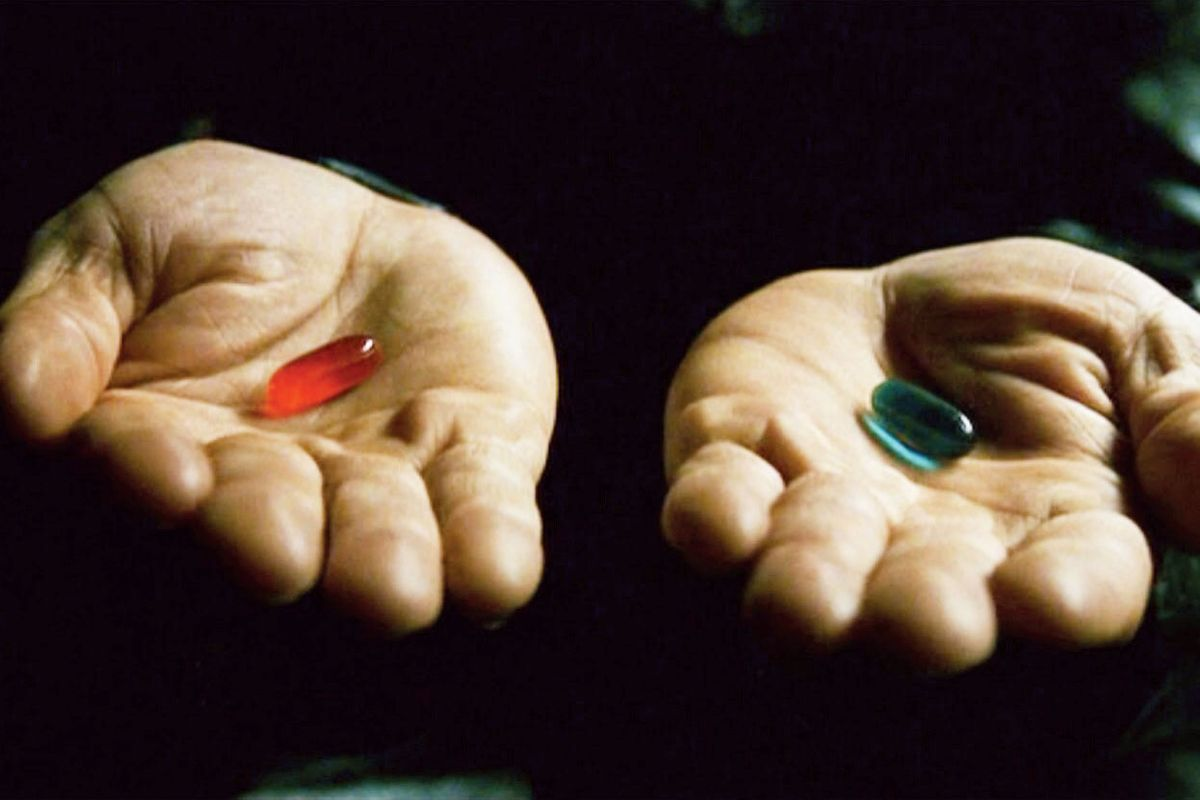
\includegraphics[width=0.5\textwidth]{MatrixPills}};
    \end{tikzpicture}
    \begin{onlyenv}<3>
        \begin{lstlisting}[style=myBash, numbers=none]
            #If session is interactive do some useful binding
            if [[ -t 1 ]]; then
                #To bind page-up and page-down to search in history
                # (command starting by what typed)
                bind '"\e[5~": history-search-backward'
                bind '"\e[6~": history-search-forward'
                #To bind up and down arrow to search in history
                # (anything containing what typed)
                bind '"\e[A": history-substring-search-backward'
                bind '"\e[B": history-substring-search-forward'
                #Move right and left one word with CTRL+@|\,\tc{red}{\ding{222}}|@ and CTRL+@|\,\tc{red}{\reflectbox{\ding{222}}}|@
                bind '"\e[1;5D": backward-word'
                bind '"\e[1;5C": forward-word'
            fi
        \end{lstlisting}
    \end{onlyenv}
    \begin{onlyenv}<4-5>
        \begin{lstlisting}[style=myBash, numbers=none, commentstyle=\color{Gray}]
            #To use global settings as well
            $include /etc/inputrc

            #To bind page-up and page-down to search in history
            # (command starting by what typed)
            |+"\e[5~": history-search-backward+|
            |+"\e[6~": history-search-forward+|
            #To bind up and down arrow to search in history
            # (anything containing what typed)
            |+"\e[A": history-substring-search-backward+|
            |+"\e[B": history-substring-search-forward+|
            #Move right and left one word with CTRL+@|\,\tc{Gray}{\ding{222}}|@ and CTRL+@|\,\tc{Gray}{\reflectbox{\ding{222}}}|@
            |+"\e[1;5D": backward-word+|
            |+"\e[1;5C": forward-word+|
        \end{lstlisting}
    \end{onlyenv}
    \FrameRemark<4-5>{Remember, you can reload the Readline init file via \texttt{CTRL-x CTRL-r} or via \,\bash|bind -f| \texttt{\textasciitilde/.inputrc} (removed commands will not be cleaned).}
\end{frame}
%~~~~~~~~~~~~~~~~~~~~~~~~~~~~~~~~~~~~~~~~~~~~%

\end{document}
